\chapter{集合论与数理逻辑}
%@see: https://plato.stanford.edu/entries/set-theory/ZF.html

\section{公理化集合论}
虽然直到19世纪末德国数学家康托才创立了集合论,
但是其实人们很早就开始使用集合的概念并对集合进行运算了.
在《周易·系辞下》中有这么一句话:“上古结绳而治,后世圣人易之以书契.”
于是我们想到,古人在农业生产中始终有着对农产品分类和计数的需要,
即将同类的产品集中地放置,
再用一个符记(例如手势、绳结、算筹、文字)表示这类产品的数量.

在本节我们先来介绍集合和元素的概念、集合存在公理,以及集合的运算法则.

\subsection{外延公理}
要实现对事物的分类,我们应该首先明白这样一点:
在现实世界中,事物之间的差异与矛盾是根本存在的.
我们知道,人对事物的认识,是人脑对客观现实的反映.
如果我们在观测事物时,观测手段十分粗略,
那么想必很难找出事物之间的差异;
如果我们在观测事物时,观测手段十分细致,
那么必然能够找出事物之间的更多差异.

为了解决上述问题,一组相对的哲学概念被提出来了,这就是“逻辑同一性”和“实在同一性”.
简单地说,实在同一性和逻辑同一性都是对事物关系的一种描述,
实在同一性要求被比较的事物无法被区分,
而逻辑同一性是指两个物在部分的属性上具备某种相同、相等或相似的关系.
以实在同一性和逻辑同一性作为分类的标准,
我们就可以区分事物以构建对立关系,又可以混同事物以构建等价关系.


\begin{axiom}[外延公理]
%@see: 《Elements of Set Theory》 P17. Extensionality Axiom
如果集合\(A\)与集合\(B\)具有相同的元素,
则称“集合\(A\)与集合\(B\)\DefineConcept{相等}”,
记作\(A=B\),即\[
	\forall A, \forall B \Bigl[
		\forall x \bigl( x \in A \iff x \in B \bigr)
		\implies A = B
	\Bigr].
\]
\end{axiom}
外延公理在英语中称作Extensionality Axiom,在德语中称作Axiom der Bestimmtheit.


\subsection{集合存在公理}
让我们想象这样的情景:
你是一个在原始部落中负责管理仓库的工人学徒.
今天,猎人们从森林里带回一些猎物,堆放在地面上,让你把它们先分好类再收进仓库.
今天是你上班的第一天,你不知道这些猎物是什么.
说要分类,你也只能一屁股坐在空地上,面朝这些码放在一起的猎物,一筹莫展.
正在此时,一位老人颤颤巍巍地走了过来,他正是你的师父.
你向他询问这些猎物应当如何分类.

“你应该首先了解这些猎物具有的特征,”
在望了一眼这堆猎物以后,你的师父说道,
“你看,和我们人类一样,这些猎物身上长着眼睛的部位也叫做头部.
在它们的头上也长有和我们的嘴巴一样用来进食的部位.
但是,你要注意,有的猎物的‘嘴’的形状与我们的嘴巴不同,它的‘嘴’是尖尖的,
我们把这类猎物的‘嘴’叫做‘喙’;
此外这类猎物也长着和我们的脚一样用来站立的部位,但它的‘脚’也是尖尖的,
我们把这类猎物的‘脚’叫做‘爪子’;
最后,我们把这类猎物叫做‘鸟’.”
他掏出水壶,喝上一口水以后,继续说:
“今天你就学习怎么把‘鸟’从这堆猎物中筛选出来,放在一起.
其余的猎物我让别人来收拾.”
紧接着,他缓缓蹲下,捡了一只长着尖喙尖爪的猎物,递给你,
“这就是‘鸟’,你照着这个样子分类吧!”
说完这句话,师父站起身来,去其他地方溜达了.

你伸出左手接住师父递给你的那只鸟,
再用空着的右手在猎物堆里扒拉,随意地拎出一只猎物.
你举起双臂,扭动翻转手腕、手肘,
仔细查看这两只猎物,比较它们的特征是否一致.
如果两者不同,右手上的猎物没有尖喙尖爪,
就把它放到身体右侧,和原本堆在地上的猎物隔开一段距离,
再用右手重新抓一只猎物进行下一轮比较;
如果两者相同,右手的猎物也有尖喙尖爪,
就把你左手提着的这只鸟放在身体左侧,也和原本堆在地上的猎物隔开一段距离,
再把右手抓着的鸟转移到左手上,
然后用右手重新抓一只猎物进行下一轮比较.

在过了一会儿后,你发现面前没有需要分类的猎物了,
于是你把左手拎着的那只鸟也放在身体左侧.
就这样,你把猎人们放在地上的那堆猎物分成了两小堆,左边这堆全是鸟.


我们经常会像上面这个故事一样,
把一些事物收集在一起,把这个整体叫做一个\DefineConcept{集合}(set),
简称为\DefineConcept{集};
然后把组成集合的这些事物叫做这个集合的\DefineConcept{元素}(member,或element),
简称为\DefineConcept{元}.
例如,在上面的故事中,在你举起双臂时,
你双手上抓着的两只鸟组成了一个集合,每只鸟都是这个集合的元素.
又例如,在你把猎物分成两堆以后,这两堆猎物中的每一堆都可以看作一个集合.
为了方便讨论,我们用大写拉丁字母(如\(A,B,C,X,Y\)等)表示集合,
用小写拉丁字母(如\(a,b,c,x,y\)等)表示元素.
由此,我们可以给出一个集合的粗糙的定义.

我们可以看出,集合具有三种特性:
\begin{enumerate}
	\item {\bf 确定性},
	即对于任意一个元素,
	要么它属于某个指定集合,
	要么它不属于该集合,
	二者必居其一.
	\begin{itemize}
		\item 如果“元素\(a\)是集合\(A\)的元素(\(a\) is a \emph{member} of \(A\),
		\(a\) is an \emph{element} of \(A\))”,
		或“\(a\)\DefineConcept{属于} \(A\)(\(a\) \emph{belongs to} \(A\))”,
		记作\(a \in A\)\footnote{%
		用来表记“所属关系(membership)”的符号\(\in\)实际上是变形的小写希腊字母\(\varepsilon\),%
		它是由皮亚诺于 1889 年提出的.}.

		\item 如果“\(b\)不是集合\(A\)的元素(\(b\) is not an element of \(A\))”,%
		或“\(b\)\DefineConcept{不属于} \(A\)(\(b\) does not belong to \(A\))”,%
		记作\(b \notin A\).
	\end{itemize}

	\item {\bf 互异性},
	即同一个集合中的元素是互不相同的,
	或者说,在以列举法表记的集合中,
	如果表记同一个元素的符号出现了多次,
	那么可以直接去除多余的符号而对集合的描述没有任何影响,即\[
		\Set{ x, x, y } = \Set{ x, y }.
	\]

	\item {\bf 无序性},
	即在以列举法表记的集合中,
	任意改变集合中元素的排列次序,
	它们仍然表示同一个集合,即\[
		\Set{ y, x } = \Set{ x, y }.
	\]
\end{enumerate}



另外,根据上面这个故事,我们还可以想到:
一方面,原本空地上没有任何我们关心的东西,至少在这里我们并不关心空气和尘土;
另一方面,对于任意两个东西,如果我们觉得这两个东西能分类在一起,就可以把它们分类在一起.
我们可以说空地是一个空着的集合,或者说“空集”.
我们还说两只鸟组成一对鸟,或者说“对集”.

从上述生活经验出发,我们认定“空集”“对集”和“并集”是一定存在的,
于是我们可以给出如下的三个公理.

\begin{axiom}[空集公理]\label{axiom:集合论.空集公理}
%@see: 《Elements of Set Theory》 P18. Empty Set Axiom
总存在这样一个集合\(A\),没有任何元素属于它\footnote{%
我们也可以用命题公式\[
	\exists A, \forall x \bigl( x \in A \iff x \neq x \bigr)
\]表示“没有任何元素的集合”的存在性.
它主要利用了“\((x \neq x)\)一定是假命题”这一点.
},即\[
	\exists A, \forall x \bigl( x \notin A \bigr).
\]
\end{axiom}

\begin{axiom}[对集公理]\label{axiom:集合论.对集公理}
%@see: 《Elements of Set Theory》 P18. Pairing Axiom
对于任意两个元素\(u\)和\(v\),
总存在一个集合\(B\),它的元素只有\(u\)和\(v\),即\[
	\forall u, \forall v, \exists B, \forall x
	\bigl(
		x \in B \iff x = u \lor x = v
	\bigr).
\]
\end{axiom}

\begin{axiom}[并集公理I]
%@see: 《Elements of Set Theory》 P18. Union Axiom, Preliminary Form
对于任意两个集合\(a\)和\(b\),
总存在一个集合\(B\),它的元素要么属于\(a\),要么属于\(b\),即\[
	\forall a, \forall b, \exists B, \forall x
	\bigl(
		x \in B
		\iff
		x \in a \lor x \in b
	\bigr).
\]
\end{axiom}

\begin{axiom}[幂集公理]
	对于任意集合\(A\),总存在一个集合\(B\),\(B\)的全部元素恰好是集合\(A\)的全部子集,即\[
	\forall A, \exists B, \forall x \bigl[
		x \in B
		\iff
		x \subseteq A
		\iff
		\forall t \bigl( t \in x \implies t \in A \bigr)
	\bigr].
\]
\end{axiom}


空集公理在英语中称作Empty Set Axiom.
对集公理在英语中称作Pairing Axiom.
并集公理在英语中称作Union Axiom, Preliminary Form,
在德语中称作Axiom der Vereinigung.
在德语中把对集公理和空集公理并称为Axiom der Elementarmengen.
幂集公理在英语中称作Power Set Axiom,在德语中称作Axiom der Potenzmenge.

下面我们给出我们对“空集”“对集”“并集”和“幂集”的正式定义.

\begin{definition}
不含任何元素的集合称为\DefineConcept{空集}(empty set),记作\(\emptyset\).
\end{definition}
%定义空集\(\emptyset\)时一定要注意两点:
%一是“空集”是否存在,这已由空集公理确保;
%二是“空集”是否唯一,这则由外延公理确保.
%若是没有这两条公理的帮助,我们就不能说\(\emptyset\)是良定义的.

\begin{definition}
对于任意给定的元素\(u\)和\(v\),
我们用符号\[
	\Set{ u, v }
\]表示只有\(u,v\)元素的集合,
并把这个集合称为“\(u\)和\(v\)的\DefineConcept{对集}(pair set)”.
\end{definition}
在对集的定义中,我们没有明确说明元素\(u,v\)是否相同.
实际上,当\(u=v\)时,\(u\)和\(v\)的对集成为只含一个元素的集合\[
	\Set{ u } = \Set{ u, v };
\]
我们称这种集合为\DefineConcept{单元素集}(singleton).
%@see: https://mathworld.wolfram.com/SingletonSet.html
单元素集是最简单的非空集合.

相对地,当\(u \neq v\)时,
我们把\(u\)和\(v\)的对集称为\DefineConcept{双元素集}.

利用对集公理和并集公理,我们可以构造任意有限集合.
例如,给定任意的\(x\),我们可以定义“单元集”如下:\[
\{x\} \defeq \{x, x\}.
\]
又例如,给定任意的\(\v{x}{3}\),我们可以定义由这三个元素构成的集合
\(\{\v{x}{3}\} \defeq \{x_1,x_2\}\cup\{x_3\}\);
同样地,我们还可以定义\(\{\v{x}{4}\}\),以此类推.

可以看出,对集公理和并集公理是保障我们采用“列举法”表示集合这一方法论的正当性的基础.


\begin{definition}
称集合\[
	\Set{ x \given x \in A \lor x \in B }
\]为“\(A\)和\(B\)的\DefineConcept{并集}(the union of \(A\) and \(B\))”,%
简称“\(A\)和\(B\)的\DefineConcept{并}”,%
记作\(A \cup B\)或\(A+B\).
\end{definition}

容易看出,当我们说“集合\(A\)不是空集”或“集合\(A\)是非空集合”时,
\(A\)中必定至少有一个元素,即\[
	\exists x \bigl( x \in A \bigr).
\]


\begin{definition}
由集合\(A\)的所有子集(包括空集和集合\(A\)本身)构成的集合\(B\),%
称作“集合\(A\)的\DefineConcept{幂集}(power set)”,%
记作\(\Powerset A\)或\(2^A\)或\(\mathcal{P}A\),即\[
	\Powerset A
	\defeq
	\Set{ x \given x \subseteq A }.
\]
\end{definition}


\begin{definition}
设系\(A = \Set{\v{a}{n}}\).
称集合\(\v{a}{n}\)的并\[
	a_1 \cup a_2 \cup \dotsb \cup a_n
\]为“\(A\)的\DefineConcept{并}”,
记作\(\bigcup A\)或\(\bigcup\limits_i a_i\),即\[
	\bigcup A
	\defeq
	a_1 \cup a_2 \cup \dotsb \cup a_n
	= \Set*{ x \given \exists a \in A \bigl( x \in a \bigr) }.
\]
\end{definition}


为了确保“系的并”这样的集合存在,我们需要改进并集公理,如下:
\begin{axiom}[并集公理II]
对于任意集合\(A\),总存在一个集合\(B\),%
使得集合\(B\)中的元素都是集合\(A\)的子集,即\[
	\forall x \Bigl[
		x \in B
		\iff
		\exists b \in A \bigl( x \in b \bigr)
	\Bigr].
\]
\end{axiom}

于是,原有的对于“集的并”的定义可以修改为\[
	a \cup b \defeq \bigcup\Set{a,b}.
\]



\begin{definition}
称集合\[
\Set{ x \given x \in A \land x \in B }
\]为“\(A\)和\(B\)的\DefineConcept{交集}(the intersection of \(A\) and \(B\))”,%
简称“\(A\)和\(B\)的\DefineConcept{交}”,%
记作\(A \cap B\)或\(AB\).
\end{definition}

\begin{theorem}\label{theorem:集合论.系的交的唯一存在性}
%@see: 《Elements of Set Theory》 P25. Theorem 2B
对于任意非空集合\(A\),%
存在唯一的集合\(B\),%
使得对于任意\(x\),有\[
	x \in B
	\iff
	\forall a \in A \bigl( x \in a \bigr).
\]
\begin{proof}
先证集合\(B\)的存在性.
既然\(A\)是非空集,不妨取定\(c \in A\).
那么根据子集公理,存在集合\(B\),使得对于任意\(x\),都有\[
	x \in B
	\iff x \in c \land \bigl[ \forall a \in A \bigl( x \in a \bigr) \bigr];
\]
由于\(c\)是任意取定的,且\[
	\bigl[ \forall a \in A \bigl( x \in a \bigr) \bigr]
	\implies
	x \in c,
\]
所以也有\[
	x \in B
	\iff \forall a \in A \bigl( x \in a \bigr).
\]

根据外延公理不难得出集合\(B\)的唯一性.
\end{proof}
\end{theorem}

\begin{definition}
称集合\[
\Set{ x \given x \in A \land x \notin B }
\]为“\(A\)和\(B\)的\DefineConcept{差集}(the relative complement of \(B\) in \(A\))”,%
记作\(A - B\)或\(A \setminus B\).
\end{definition}

\begin{example}
%@see: 《Elements of Set Theory》 P26. Example
如果\(b \in A\),那么\(b \subseteq \bigcup A\).
\end{example}

\begin{example}\label{example:集合论.有序对各坐标的取值范围}
%@see: 《Elements of Set Theory》 P26. Example
%@see: 《Elements of Set Theory》 P38. Lemma 3D
如果有\(\Set{ \Set{x}, \Set{x,y} } \in A\),
考虑到\(\Set{x,y} \in \Set{ \Set{x}, \Set{x,y} }\),
那么有\[
	\Set{x,y} \in \bigcup A;
\]
再考虑到\(x,y \in \Set{x,y}\),
进而有\[
	x,y \in \bigcup\bigcup A.
\]
综上所述,我们有
\begin{equation}
	\Set{ \Set{x}, \Set{x,y} } \in A
	\implies
	x,y \in \bigcup\bigcup A.
\end{equation}
\end{example}

\begin{example}
%@see: 《Elements of Set Theory》 P26. Example
因为\[
	\bigcap\Set{\Set{a},\Set{a,b}}
	= \Set{a}\cap\Set{a,b}
	= \Set{a},
\]
所以\[
	\bigcup\bigcap\Set{\Set{a},\Set{a,b}}
	= \bigcup\Set{a}
	= a.
\]

类似有\[
	\bigcap\bigcup\Set{\Set{a},\Set{a,b}}
	= \bigcap\Set{a,b}
	= a \cap b.
\]
\end{example}


\begin{definition}
设系\(A = \Set{\v{a}{n}}\).
称集合\(\v{a}{n}\)的交\[
	a_1 \cap a_2 \cap \dotsb \cap a_n
\]为\(A\)的\DefineConcept{交}\footnote{%
\cref{theorem:集合论.系的交的唯一存在性} 确保了\(\bigcap A\)可以定义为唯一存在的集合\(B\).
},%
记作\(\bigcap A\)或\(\bigcap\limits_i a_i\),即\[
	\bigcap A
	\defeq
	a_1 \cap a_2 \cap \dotsb \cap a_n
	= \Set*{ x \given \forall a \in A \bigl(x \in a\bigr) }.
\]
\end{definition}

例如,
\begin{align*}
	&\bigcup\Set{a,b,c,d} = a \cup b \cup c \cup d. \\
	&\bigcup\Set{a} = a. \\
	&\bigcup\emptyset = \emptyset.
\end{align*}

例如,
\begin{align*}
	&\bigcap\Set{a} = a. \\
	&\bigcap\Set{a,b} = a \cap b. \\
	&\bigcap\Set{a,b,c,d} = a \cap b \cap c \cap d.
\end{align*}

特别注意到“\(\bigcap\emptyset\)”是未定义的!

\begin{example}
因为\(\bigcap\Set{ \Set{a}, \Set{a,b} } = \Set{a} \cap \Set{a,b} = \Set{a}\),%
所以\[
\bigcup \bigcap \Set{ \Set{a}, \Set{a,b} } = \bigcup \Set{a} = a;
\]\[
\bigcap \bigcup \Set{ \Set{a}, \Set{a,b} } = \bigcap \Set{a,b} = a \cap b.
\]
\end{example}


\begin{property}
%@see: 《Elements of Set Theory》 P26. Exercise 6(a).
对任意集合\(A\),总有
\begin{equation}
	\bigcup \Powerset A = A.
\end{equation}
\begin{proof}
令\(B = \Powerset A\).
由并集的定义可知,\[
	x \in \bigcup B
	\iff
	\exists b \in B
	\bigl(
		x \in b
	\bigr).
	\eqno(1)
\]
又由幂集的定义可知,\[
	b \in B = \Powerset A
	\iff
	b \subseteq A.
	\eqno(2)
\]
结合(1)式与(2)式,可知\[
	x \in \bigcup \Powerset A
	\iff
	\exists b \subseteq A
	\bigl(
		x \in b
	\bigr).
	\eqno(3)
\]
于是,若要证\(\bigcup \Powerset A = A\),
只需证\(x \in \bigcup \Powerset A \iff x \in A\),
即证\[
	x \in A
	\iff
	\exists b \subseteq A
	\bigl(
		x \in b
	\bigr).
	\eqno(4)
\]
(4)式是显然的.
\end{proof}
\end{property}


\begin{example}
%@see: 《Elements of Set Theory》 P26. Exercise 6(b).
证明:对任意集合\(A\),总有
\begin{equation}
	A \subseteq \Powerset \bigcup A;
\end{equation}
并找出使得\(A = \Powerset \bigcup A\)成立的条件.
%TODO
\end{example}



\subsection{子集公理}
\begin{axiom}[子集公理]
%@see: 《Elements of Set Theory》 P21. Subset Axiom
对于不涉及\(B\)的每一条命题公式\(\lambda\),命题\[
	\forall A, \exists B, \forall x \bigl(
		x \in B \iff x \in A \land \lambda
	\bigr)
\]是一条公理.
\end{axiom}
子集公理有时候也称作\DefineConcept{分离公理},%
它在英语中称作Subset Axioms,%
在德语中称作Axiom der Aussonderung.
正如其名,该定理的作用就是从集合\(A\)中取出适合命题公式\(\lambda\)的元素,组合成新的集合\(B\).

可以看出,子集公理是保障我们采用“描述法”表示集合这一方法论的正当性的基础.
也就是说,\[
\Bigl[
	\forall A, \exists B, \forall x \bigl(
		x \in B \iff x \in A \land \lambda
	\bigr)
\Bigr]
\quad\iff\quad
B = \Set{ x \in A \given \lambda }.
\]

利用描述法,我们可以重新定义空集如下:\[
	\emptyset \defeq \Set{ x \given x \neq x }.
\]

\begin{example}
以空集为元素构成的集合\(\Set{\emptyset}\)不是空集,即\(\Set{\emptyset} \neq \emptyset\).
这是因为\(\emptyset \in \Set{\emptyset}\)但\(\emptyset \notin \emptyset\).
\end{example}


\begin{theorem}\label{theorem:集合论.以所有集合为元素组成的集合不存在}
%@see: 《Elements of Set Theory》 P22. Theorem 2A
以所有集合为元素组成的集合不存在.
\begin{proof}
设\(A\)是一个集合.
令\[
B = \Set{ x \in A \given x \notin x }.
\]那么有\[
B \in B
\iff
B \in A \land B \notin B.
\eqno(1)
\]

假设\(B \in A\),那么(1)式化为\[
B \in B \iff B \notin B,
\]矛盾,故\(B \notin A\).

综上所述,我们总可构造出一个不属于\(A\)的集合\(B\),因此不存在“以所有集合为元素组成的集合”.
\end{proof}
\end{theorem}
有的人可能会对是否存在以其本身为元素的集合抱有疑问,我们将在后面证明这是不可能的.
而根据这个结论,在上面的证明中,集合\(B\)实际上与集合\(A\)完全相同.

利用子集定理,我们可以进一步定义子集、真子集、交集等概念.
\begin{definition}
设\(A\)、\(B\)是两个集合,如果集合\(A\)的元素都是集合\(B\)的元素,则称“\(A\)是\(B\)的\DefineConcept{子集}(\(A\) is a \emph{subset} of \(B\))”,%
记作\(A \subseteq B\)读作“\(A\)包含于\(B\)(\(A\) is included in \(B\))”,%
或记作\(B \supseteq A\)读作“\(B\)包含\(A\)(\(B\) includes \(A\))”,%
即\[
\forall x \in A \bigl( x \in B \bigr)
\iff A \subseteq B
\iff B \supseteq A.
\]

若集合\(A \subseteq B\)且\(A \neq B\),则称“\(A\)是\(B\)的\DefineConcept{真子集}(\(A\) is a \emph{proper subset} of \(B\))”,记作\(A \subsetneqq B\)读作“\(A\)是\(B\)的真子集”.
\end{definition}

\begin{theorem}
任意集合都是其本身的子集,即\[
\forall A \bigl( A \subseteq A \bigr).
\]
\end{theorem}

\begin{theorem}
空集\(\emptyset\)是任何集合的子集,即\[
\forall A \bigl( \emptyset \subseteq A \bigr);
\]还是任何非空集合的真子集,即\[
\forall A \bigl( A \neq \emptyset \iff \emptyset \subsetneqq A \bigr).
\]
\end{theorem}

在学习了从属关系(\(\in\))和包含关系(\(\subseteq\))以后,切莫将两者搞混.
在讨论\(A \in B\)是否成立时,我们是将\(A\)作为一个整体,看它是不是\(B\)中的一个元素.
在讨论\(A \subseteq B\)是否成立时,我们要将\(A\)打开,检查它里面的所有元素是不是都是\(B\)中的元素.

\begin{theorem}
如果集合\(A\)与集合\(B\)互为子集,那么集合\(A\)与集合\(B\)相等,即\[
A \subseteq B \land B \subseteq A
\iff
A = B.
\]
\end{theorem}

\begin{example}
\(\Powerset \emptyset = \{ \emptyset \},%
\Powerset \Set{ \emptyset } = \{ \emptyset, \{ \emptyset \} \}\).
\end{example}

\begin{example}
对于任意集合\(A,B\),试分析\(\Powerset(A-B)\)与\(\Powerset A - \Powerset B\)是否相等.
\begin{solution}
集合\(\Powerset(A-B)\)包含集合\(A-B\)的所有子集,那么总有\(\emptyset\in\Powerset(A-B)\).
但是\(\emptyset\notin\Powerset A - \Powerset B\),所以\(\Powerset(A-B) \neq \Powerset A - \Powerset B\).
\end{solution}
\end{example}

\begin{example}
求非空集合\(S\)的所有单元素子集.
\begin{solution}
我们知道\(\Powerset S\)中的元素是\(S\)的全部子集,
于是我们可以利用子集公理从中找出只有一个元素的集合,将它们重组为一个新的集合\[
	\Set{ a \in \Powerset S \given a\text{是单元集} }.
\]
我们知道,单元素集中有且仅有一个元素,由此可知\[
	a \neq \emptyset
	\land
	\forall u,v \in a \bigl( u = v \bigr).
\]
综上所述,非空集合\(S\)的所有单元素子集的集合为\[
	\Set*{ a \in \Powerset S \given a \neq \emptyset
	\land
	\forall u,v \in a \bigl( u = v \bigr) }.
\]
\end{solution}
\end{example}

\subsection{集合代数}
\begin{definition}[全集、补集]
有时,我们研究某个问题限定在一个大的集合\(U\)中进行,所研究的其他集合都是\(U\)的子集;
此时我们称集合\(U\)为\DefineConcept{全集}(universe)或\DefineConcept{基本集}.

设集合\(A \subseteq U\),则称\(U-A\)为\(A\)的\DefineConcept{补集}或\DefineConcept{余集},记作\(\overline{A}\),或\(\complement_U A\),或\(A^C\).
\end{definition}

\begin{theorem}
对于任意非空集合\(A\),总存在唯一的集合\(B\),使得\[
\forall x \bigl[
	x \in B \iff (\forall a \in A) x \in a
\bigr].
\]
\begin{proof}
从非空集合\(A\)中任取一个元素\(c\).
根据子集公理,存在集合\(B\)使得\[
\forall x \left[
	\begin{array}{rl}
	x \in B &\iff x \in c \land (\forall a \in A) x \in a \\
		&\iff (\forall a \in A) x \in a
	\end{array}
\right].
\]唯一性可通过外延公理证明.
\end{proof}
\end{theorem}


\begin{figure}[ht]
	\def\subwidth{.5\linewidth}
	\centering
	\begin{subfigure}[b]{\subwidth}
		\centering
		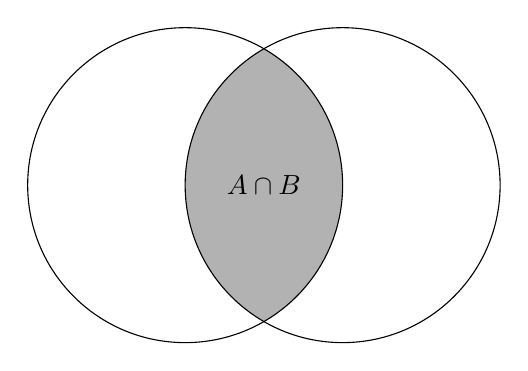
\begin{tikzpicture}
			\path[save path=\pathA](-1,0)circle(2cm);
			\path[save path=\pathB](+1,0)circle(2cm);
			\begin{scope}
				\clip[use path=\pathA];
				\fill[black!30][use path=\pathB];
			\end{scope}
			\draw[use path=\pathA];
			\draw[use path=\pathB];
			\draw(0,0)node{\(A \cap B\)};
		\end{tikzpicture}
		\subcaption{集合的交}
	\end{subfigure}%
	\begin{subfigure}[b]{\subwidth}
		\centering
		\begin{tikzpicture}
			\path[save path=\pathA,name path=A](-1,0)circle(2cm);
			\path[save path=\pathB,name path=B](+1,0)circle(2cm);
			\path[fill=black!30][use path=\pathA+\pathB];
			\draw[name intersections={of=A and B}]
				(intersection-1)arc[start angle=60,end angle=300,radius=2]
				(intersection-2)arc[start angle=-120,end angle=120,radius=2]
				(intersection-1);
			\draw(0,0)node{\(A \cup B\)};
			\pgfresetboundingbox
			\path[use as bounding box] (-3,-2)rectangle(3,2);
		\end{tikzpicture}
		\subcaption{集合的并}
	\end{subfigure}%

	\begin{subfigure}[b]{\linewidth}
		\centering
		\begin{tikzpicture}
			\path[save path=\pathA,name path=A](-1,0)circle(2cm);
			\path[save path=\pathB,name path=B](+1,0)circle(2cm);
			\begin{scope}
				\clip[name intersections={of=A and B}]
					(intersection-1)arc[start angle=60,end angle=300,radius=2]
					(intersection-2)arc[start angle=-120,end angle=-240,radius=2]
					(intersection-2);
				\fill[black!30][use path=\pathA];
			\end{scope}
			\draw[use path=\pathA];
			\draw[use path=\pathB];
			\draw(-2,0)node{\(A-B\)};
			\pgfresetboundingbox
			\path[use as bounding box] (-3,-2)rectangle(3,2);
		\end{tikzpicture}
		\subcaption{集合的差}
	\end{subfigure}%
	\caption{韦恩图}
	\label{figure:集合论.韦恩图}
\end{figure}

\begin{property}
集合的运算满足以下性质:
\begin{enumerate}
\item 交换律({\rm Commutative laws})
\begin{gather}
A \cap B = B \cap A, \label{equation:集合论.集合代数公式1} \\
A \cup B = B \cup A. \label{equation:集合论.集合代数公式2}
\end{gather}

\item 结合律({\rm Associative laws})
\begin{gather}
(A \cap B) \cap C = A \cap (B \cap C), \label{equation:集合论.集合代数公式3} \\
(A \cup B) \cup C = A \cup (B \cup C). \label{equation:集合论.集合代数公式4}
\end{gather}

\item 分配律({\rm Distributive laws})
\begin{gather}
(A \cap B) \cup C = (A \cup C) \cap (B \cup C), \label{equation:集合论.集合代数公式5} \\
(A \cup B) \cap C = (A \cap C) \cup (B \cap C), \label{equation:集合论.集合代数公式6} \\
A \cup \bigcap \mathscr{B} = \bigcap\Set{A \cup X \given X \in \mathscr{B}} \quad(\mathscr{B}\neq\emptyset), \label{equation:集合论.集合代数公式5'} \\
A \cap \bigcup \mathscr{B} = \bigcup\Set{A \cap X \given X \in \mathscr{B}}. \label{equation:集合论.集合代数公式6'}
\end{gather}

\item 对偶律({\rm De Morgan's laws})(假设\(\mathscr{A}\neq\emptyset\))
\begin{gather}
\overline{A \cap B} = \overline A \cup \overline B, \label{equation:集合论.集合代数公式7} \\
\overline{A \cup B} = \overline A \cap \overline B, \label{equation:集合论.集合代数公式8} \\
C - \bigcup\mathscr{A} = \bigcap\Set{C-X \given X\in\mathscr{A}}, \label{equation:集合论.集合代数公式7'} \\
C - \bigcap\mathscr{A} = \bigcup\Set{C-X \given X\in\mathscr{A}}. \label{equation:集合论.集合代数公式8'}
\end{gather}

\item 与空集\(\emptyset\)和全集\(\Omega\)的运算(假设\(A \subseteq \Omega\))
\begin{gather}
A \cup \emptyset = A, \label{equation:集合论.集合代数公式9} \\
A \cap \emptyset = \emptyset, \label{equation:集合论.集合代数公式10} \\
A \cup \Omega = \Omega, \label{equation:集合论.集合代数公式11} \\
A \cap \Omega = A, \label{equation:集合论.集合代数公式12} \\
A \cup \overline{A} = \Omega, \label{equation:集合论.集合代数公式13} \\
A \cap \overline{A} = \emptyset. \label{equation:集合论.集合代数公式14}
\end{gather}

\item 包含关系的单调性
\begin{gather}
A \subseteq B \implies A \cup C \subseteq B \cup C, \label{equation:集合论.集合代数公式15} \\
A \subseteq B \implies A \cap C \subseteq B \cap C, \label{equation:集合论.集合代数公式16} \\
A \subseteq B \implies \bigcup A \subseteq \bigcup B, \label{equation:集合论.集合代数公式17} \\
A \subseteq B \implies \overline{B} \subseteq \overline{A}, \label{equation:集合论.集合代数公式18} \\
\emptyset \neq A \subseteq B \implies \bigcap B \subseteq \bigcap A. \label{equation:集合论.集合代数公式19}
\end{gather}
\end{enumerate}
\begin{proof}
对于\cref{equation:集合论.集合代数公式19},假设\(x \in A = \Set{\v{a}{0}} \implies x \in B = \Set{\v{b}{0}}\),%
那么
\begin{align*}
x \in \bigcap B = \bigcap_i b_i
&\iff
	x \in b_i\ (i=1,2,\dotsc) \\
&\implies
	x \in a_i\ (i=1,2,\dotsc) \\
&\iff
	x \in \bigcap_i a_i = \bigcap A.
\qedhere
\end{align*}
\end{proof}
\end{property}

\begin{example}
证明:\((A \cup B) - (A \cap B) = (A-B)\cup(B-A)\).
\begin{proof}
根据集合交、并、差的定义,有
\begin{align*}
&\hspace{-20pt}
(A \cup B) - (A \cap B) \\
&= \Set{ x \given x \in (A \cup B) \land x \notin (A \cap B) } \\
&= \Set{ x \given (x \in A \lor x \in B) \land \neg(x \in A \land x \in B) } \\
&= \Set{ x \given [x \in A \land \neg(x \in A \land x \in B)]
 \lor [x \in B \land \neg(x \in A \land x \in B)] } \\
&= \Set{ x \given [x \in A \land (x \notin A \lor x \notin B)]
 \lor [x \in B \land (x \notin A \lor x \notin B)] } \\
&= \Set{ x \given (x \in A \land x \notin B) \lor (x \in B \land x \notin A) } \\
&= (A-B)\cup(B-A).
\qedhere
\end{align*}
\end{proof}
\end{example}

\section{关系}
\subsection{无序对、有序对的概念}
\begin{definition}[无序对]
由两个元素\(x_1\)和\(x_2\)组成的集合\[
\Set{x_1, x_2}
\]称作\DefineConcept{无序对}(unordered pair).
\end{definition}

\begin{example}
%@see: 《Elements of Set Theory》 P38. Exercise 1.
定义:\[
\opair{x,y,z}^* = \{\{x\},\{x,y\},\{x,y,z\}\}.
\]找出元素\(u,v,w,x,y,z\)使\[
\opair{x,y,z}^* = \opair{u,v,w}^*
\]成立,但\(y \neq v\)或\(z \neq w\).
\begin{solution}
取\[
\opair{1,1,2}^* = \{\{1\},\{1,1\},\{1,1,2\}\} = \{\{1\},\{1,2\}\},
\]\[
\opair{1,2,1}^* = \{\{1\},\{1,2\},\{1,2,1\}\} = \{\{1\},\{1,2\}\},
\]即可满足题设条件.
\end{solution}
\end{example}

\begin{definition}[有序对]
两个元素\(x_1\)和\(x_2\)按一定顺序形成的排列称为\DefineConcept{有序对},记作\[
\opair{x_1,x_2}.
\]

我们可以采用多种方式构造集合用于表记有序对\(\opair{x_1,x_2}\),例如(由Norbert Wiener于1914年构造的)
\[
\Set{ \Set{ \Set{x_1}, \emptyset }, \Set{ \Set{ x_2 } } }.
\]
但我们更常用(由Kazimierz Kuratowski于1921年构造的)以下形式
\[
\Set{ \Set{x_1}, \Set{x_1, x_2} }.
\]以后我们都采用第二种形式表记有序对,因此\[
\opair{x_1,x_2}
\defeq
\Set{ \Set{x_1}, \Set{x_1, x_2} }.
\]
\end{definition}

有序对具有以下性质.
\begin{property}\label{theorem:集合论.有序对的性质1}
%@see: 《Elements of Set Theory》 P36. Theorem 3A
\(\opair{u,v} = \opair{x,y}\)的充要条件是:\(u=x\)且\(v=y\).
\begin{proof}
充分性.
这个方向的证明是平凡的;
当\(u=x\)且\(v=y\)时,自然有\[
	\opair{u,v} = \opair{x,y}.
\]

必要性.
当\(\opair{u,v} = \opair{x,y}\)时,根据定义有\[
	\Set{ \Set{u}, \Set{u, v} }
	= \Set{ \Set{x}, \Set{x, y} };
\]于是\[
	\Set{u} \in \Set{ \Set{x}, \Set{x, y} },
	\eqno{(1)}
\]且\[
	\Set{u,v} \in \Set{ \Set{x}, \Set{x, y} }.
	\eqno{(2)}
\]
从(1)式我们知道,要么等式\[
	\Set{u} = \Set{x}
	\eqno{(3)}
\]成立,要么等式\[
	\Set{u} = \Set{x,y}
	\eqno{(4)}
\]成立;
从(2)式我们知道,要么等式\[
	\Set{u,v} = \Set{x}
	\eqno{(5)}
\]成立,要么等式\[
	\Set{u,v} = \Set{x,y}
	\eqno{(6)}
\]成立.

首先我们假设(4)式成立,那么有\(u = x = y\);
从而有(5)式等价于(6)式,且\(u = v = x = y\);
在这种情况下,必要性得证.
同理,假设(5)式成立,也可证明必要性.

然后我们假设(3)式、(6)式同时成立.
从(3)式成立我们知道\(u = x\).
从(6)式成立我们知道\(u = y\)或\(v = y\);
第一种情况,即\(u = x\)和\(u = y\)同时成立的情况,已经在(4)式成立时作了讨论.
第二种情况,即\(u = x\)和\(v = y\)同时成立的情况,立即保证了必要性.
\end{proof}
\end{property}
\cref{theorem:集合论.有序对的性质1} 让我们可以不含糊地将有序对\(\opair{x,y}\)
中的\(x\)和\(y\)分别称为%
有序对的\DefineConcept{第一坐标}(first coordinate)%
和\DefineConcept{第二坐标}(second coordinate).

\subsection{直积}
\begin{definition}[直积]\label{definition:集合论.直积}
设\(A,B\)都是集合.
在\(A\)中任取一个元素\(x\),
在\(B\)中任取一个元素\(y\),
组成一个有序对\(\opair{x,y}\),
把这样的有序对作为新的元素,
它们全体组成的集合称为“\(A\)与\(B\)的%
\DefineConcept{直积}或\DefineConcept{笛卡尔乘积}(Cartesian product)”,
记为\(A \times B\),即\[
	A \times B
	\defeq
	\Set{ \opair{x,y} \given x \in A, y \in B }.
\]

特别地,集合\(A\)与自己的直积\(A \times A\)可以简记为\(A^2\),
\((A \times A) \times A\)可以简记为\(A^3\),以此类推.
\end{definition}

在宣称\cref{definition:集合论.直积} 合法以前,
我们必须确认它给出的收集\(A \times B\)是不是真的是一个集合.
我们在运用描述法记号\[
	\Set{ t \given \lambda(t) }
\]表记一个集合时,必须验证是不是真的存在一个集合\(D\),使得\[
	\forall t \bigl( t \in D \iff \lambda(t) \bigr)
\]成立,其中\(\lambda(t)\)表示与\(t\)有关的命题公式.
例如,虽然\[
	\Set{ x \given x = x }
	\quad\text{和}\quad
	\Set{ x \given x \neq x }
\]这两个表达式看起来相似,
但根据\cref{theorem:集合论.以所有集合为元素组成的集合不存在},
这里的第一个表达式不能表示一个集合;
然而根据空集公理,第二个表达式就可以表示空集.

要证明\(A \times B\)是一个集合,
我们就必须找到一个足够大的集合,
它包括了我们需要的全部有序对,
然后利用子集公理证明\(A \times B\)是这个集合的子集.
因此,我们给出下述引理.
\begin{lemma}\label{theorem:集合论.有序对是其坐标元素所在集合的二重幂集的元素}
%@see: 《Elements of Set Theory》 P37. Lemma 3B
如果\(x,y \in A\),那么\[
	\opair{x,y} \in \Powerset\Powerset A.
\]
\begin{proof}
由\(x,y \in A\)可知\(\{x\},\{x,y\} \subseteq A\),
即\(\{x\},\{x,y\} \in \Powerset A\),
那么\(\{\{x\},\{x,y\}\} \subseteq \Powerset A\),
进一步可得\(\{\{x\},\{x,y\}\} \in \Powerset\Powerset A\).
\end{proof}
\end{lemma}

\begin{theorem}\label{theorem:集合论.直积存在定理}
%@see: 《Elements of Set Theory》 P38. Corollary 3C
对任意集合\(A,B\),存在这样一个集合,
它的元素全是有序对\(\opair{x,y}\),
其中\(x \in A\),\(y \in B\).
\begin{proof}
根据子集公理,我们可以构造集合\[
	\Set*{ w \in \Powerset\Powerset(A \cup B) \given w = \opair{x,y}, x \in A, y \in B }.
\]
显然,根据\cref{theorem:集合论.有序对是其坐标元素所在集合的二重幂集的元素},
这个集合仅包括我们需要的有序对.
\end{proof}
\end{theorem}
依靠\cref{theorem:集合论.直积存在定理},
我们就可以正当化先前对\hyperref[definition:集合论.直积]{直积}\(A \times B\)的定义.

容易发现,对于任意集合\(A\),总有\begin{equation}
	A \times \emptyset
	= \emptyset \times A
	= \emptyset \times \emptyset
	= \emptyset.
\end{equation}

\begin{example}
%@see: 《Elements of Set Theory》 P38. Exercise 2.(a)
证明:\begin{equation}
	A \times (B \cup C) = (A \times B) \cup (A \times C).
\end{equation}
\begin{proof}
由于对于任意\(w = \opair{x,y}\)总有
\begin{align*}
	w \in A \times (B \cup C)
	&\iff x \in A \land y \in B \cup C \\
	&\iff x \in A \land (y \in B \lor y \in C) \\
	&\iff x \in A \land y \in B \lor x \in A \land y \in C \\
	&\iff w \in A \times B \lor w \in A \times C,
\end{align*}
那么由外延公理可知\(A \times (B \cup C) = (A \times B) \cup (A \times C)\).
\end{proof}
\end{example}

\begin{example}
%@see: 《Elements of Set Theory》 P38. Exercise 2.(b)
证明:如果\(A \times B = A \times C\)且\(A \neq \emptyset\),则\(B = C\).
%TODO
\end{example}

\begin{example}
%@see: 《Elements of Set Theory》 P38. Exercise 3.
证明:\(A \times \bigcup B = \bigcup\Set{ A \times X \given X \in B }\).
%TODO
\end{example}

\begin{example}
%@see: 《Elements of Set Theory》 P38. Exercise 5.(a)
设\(A,B\)都是集合,试证:\(\Set{ \{x\} \times B \given x \in A }\)也是集合.
%TODO
\end{example}

\subsection{关系}
\begin{definition}
\DefineConcept{关系}(relation)是有序对的集合.
\end{definition}

如果有序对\(\opair{x,y}\)是关系\(\rel{R}\)的元素,即\[
	\opair{x,y} \in \rel{R},
\]
那么称“\(x\)与\(y\)有\(\rel{R}\)关系”,
记作\(x\rel{R}y\);
反之,\[
	\opair{x,y} \notin \rel{R},
\]
那么称“\(x\)与\(y\)没有\(\rel{R}\)关系”.

给定集合\(X\)和集合\(Y\),
如果关系\(\rel{R}\)满足\[
	\rel{R} \subseteq X \times Y,
\]
我们就称“\(\rel{R}\)是\(X\)与\(Y\)之间的\DefineConcept{二元关系}(binary relation)”.
特别地,当\(X = Y\)时,就称“\(\rel{R}\)是\(X\)上的\DefineConcept{二元关系}”.

从关系的定义可以看出,关系是有序对的集合.
即便是看起来毫无意义的,只由一个有序对组成的集合,也可以看成是一个关系.
我们自然会认为有的关系比别的关系更有意义,
例如我们马上会提到的“映射”“等价关系”和“偏序关系”.

\begin{definition}\label{definition:集合论.定义域与值域的定义}
设\(R\)是集合.

如果集合\(A\)满足\[
	x \in A \iff \exists y \bigl( \opair{x,y} \in R \bigr),
\]
那么称\(A\)为“\(R\)的\DefineConcept{定义域}(domain)”,记作\(\dom R\).

如果集合\(B\)满足\[
	x \in B \iff \exists t \bigl( \opair{t,x} \in R \bigr),
\]
那么称\(B\)为“\(R\)的\DefineConcept{值域}(range)”,记作\(\ran R\).

最后,我们把\(R\)的定义域与它的值域的并集称为
“\(R\)的\DefineConcept{域}(field)”,记作\(\fld R\),即\[
	\fld R \defeq \dom R \cup \ran R.
\]
\end{definition}

为了正当化\cref{definition:集合论.定义域与值域的定义},
我们必须明确:对于任意集合\(R\),存在这样一个集合,
\(R\)中的有序对的第一坐标和第二坐标都是这个集合的元素.
这个问题类似于我们之前对于直积\(A \times B\)的定义的正当化,
当时我们证明了\cref{theorem:集合论.直积存在定理}.
为此,我们给出下述引理,
可以注意到它与\cref{theorem:集合论.有序对是其坐标元素所在集合的二重幂集的元素} 的关联.

\begin{lemma}
%@see: 《Elements of Set Theory》 P38. Lemma 3D
如果\(\opair{x,y} \in A\),那么\(x,y \in \bigcup\bigcup A\).
\end{lemma}
这条引理已经在\cref{example:集合论.有序对各坐标的取值范围} 得到证明.
利用这条引理,再加上子集公理,我们可以构造集合\(R\)的定义域和值域:
\begin{gather}
	\dom R
	\defeq
	\Set*{ x \in \bigcup\bigcup R \given \exists y \bigl( \opair{x,y} \in R \bigr) }, \\
	\ran R
	\defeq
	\Set*{ x \in \bigcup\bigcup R \given \exists t \bigl( \opair{t,x} \in R \bigr) }.
\end{gather}

\begin{example}
%@see: 《Elements of Set Theory》 P41. Exercise 6.
试证:集合\(A\)是一个关系的充要条件是\[
	A \subseteq \dom A \times \ran A.
\]
%TODO
\end{example}

\begin{example}
%@see: 《Elements of Set Theory》 P41. Exercise 7.
试证:给定关系\(\rel{R}\),总有\[
	\fld \rel{R} = \bigcup\bigcup \rel{R}.
\]
%TODO
\end{example}

\begin{example}
%@see: 《Elements of Set Theory》 P41. Exercise 8.
试证:对于任意集合\(A\),总有\begin{gather}
	\dom\bigcup A = \bigcup\Set{ \dom\rel{R} \given \rel{R} \in A }, \\
	\ran\bigcup A = \bigcup\Set{ \ran\rel{R} \given \rel{R} \in A }.
\end{gather}
%TODO
\end{example}

\subsection{多元关系}
我们可以将“有序对”和“二元关系”的概念分别扩展为“元组”和“多元关系”.

例如定义\[
	\opair{x_1,x_2,x_3}
	\defeq
	\opair{\opair{x_1,x_2},x_3},
\]
称之为\DefineConcept{三元组}(triple);
定义\[
	\opair{x_1,x_2,x_3,x_4}
	\defeq
	\opair{\opair{x_1,x_2,x_3},x_4},
\]
称之为\DefineConcept{四元组}(quadruple);
定义\[
	\opair{x_1,x_2,x_3,x_4,x_5}
	\defeq
	\opair{\opair{x_1,x_2,x_3,x_4},x_5},
\]
称之为\DefineConcept{五元组}(quintuple);
以此类推,对于任意给定\(n\),可以定义\(n\)元组(\(n\)-tuple):\[
	\opair{x_1,x_2,\dotsc,x_n}
	\defeq
	\opair{\opair{x_1,x_2,\dotsc,x_{n-1}},x_n}.
\]
为了让我们的定义看起来整齐划一,我们还可以补充定义\[
	\opair{x} \defeq x,
\]
称之为\DefineConcept{一元组}(1-tuple).

我们把“在\(A\)上的\(n\)元\DefineConcept{关系}(n-ary \emph{relation} on \(A\))”%
定义为由\(n\)元组构成的集合.
由于\(A\)上的二元关系是\(A \times A\)的子集,
以及\(A\)上的三元关系(ternary relation, 3-ary relation)是\((A \times A) \times A\)的子集,
所以三元关系也可归结为一种二元关系;
同理,其他\(n\)元关系,只要\(n>1\),也都可以归结为二元关系.
虽然在上面对\(n\)元关系的定义中,
我们也把由\(A\)中包括的一元组构成的集合称为%
“\(A\)上的一元关系(unary relation, 1-ary relation)”,
但它只是\(A\)的一个子集,根本不满足关系的定义.

\section{映射}
\subsection{映射的概念}
\begin{definition}
设\(F\)是关系,如果\[
	\forall x \in \dom F, \exists! y:
	x F y,
\]
则称“关系\(F\)是一个\DefineConcept{映射}(function)”.
\end{definition}
可以从映射的定义中看出,虽然映射也是关系,
但映射有一般的关系所没有的特殊性质:
映射是\DefineConcept{单值的}(single-valued).
换句话说,对于关系\(F\),每个\(x\)可能对应若干个\(y\);
但是,对于映射\(F\),每个\(x\)就只对应一个\(y\).
我们可以把\(x\)与\(y\)这两个元素之间的对应关系记为\(x \mapsto y\).

我们把使得\(xFy\)成立的\(y\)称为“\(x\)(在映射\(F\)下)的\DefineConcept{像}%
(the \emph{value} of \(F\) at \(x\))”,
记为\(F(x)\),即\[
	y = f(x);
\]
称\(x\)为“\(y\)(在映射\(F\)下)的一个\DefineConcept{原像}”.
这里用的\(F(x)\)符号是欧拉提出的,
我们仅当\(F\)是一个映射且\(x\in\dom F\)时使用这个记号.
不过,我们也可以定义:\[
	F(x) \defeq \bigcup\Set{ y \given \opair{x,y} \in F }.
\]
它对于任意\(F\)和\(x\)都有意义.

映射是如此重要,以至于各家对用于描述映射的术语没有达成统一.
以下是两种最常采用的术语.

设\(X,Y\)都是集合,
如果\(f\)是一个映射,且\(\dom f = X\),\(\ran f \subseteq Y\),
则称“\(f\)是从\(X\)到\(Y\)的\DefineConcept{映射}%
(\(f\) is a function \emph{from} \(X\) \emph{into} \(Y\))”,
或称“\(f\)将\(X\)映射到\(Y\)里%
(\(f\) \emph{maps} \(X\) \emph{into} \(Y\))”,
记作\[
	f\colon X \to Y.
\]
如果还有\(\ran f = Y\),
那么称“\(f\)是从\(X\)到\(Y\)上的映射%
(\(f\) is a function from \(X\) \emph{onto} \(Y\))”,
或称“\(f\)将\(X\)映射到\(Y\)上%
(\(f\) \emph{maps} \(X\) \emph{onto} \(Y\))”.
我们可以说“任意映射总将它的定义域映射到它的值域上”,
还可以说“任意映射总把它的定义域映射到以它的值域为子集的任意集合\(B\)里”.
注意到两种说法的区别,“上”字和“里”字的选用,
不光取决于映射\(f\)本身,还取决于我们讨论的集合\(B\).

如果\[
	\forall y \in \ran f,
	\exists! x:
	x f y,
\]
那么称“映射\(f\)是\DefineConcept{一一映射}(one-to-one)”.

有时候我们希望把一一映射的概念套用到一般的关系上,
它们往往不是映射,因此“一一映射”这个用词就显得不那么恰当了.
为此,我们创造出“单根的”,类比于“单值的”.

\begin{definition}
如果集合\(R\)满足\[
	\forall y \in \ran R,
	\exists! x:
	x R y,
\]
则称“\(R\)是\DefineConcept{单根的}(single-rooted)”.
\end{definition}

因此,我们可以说,“一个映射是单根的”当且仅当“这个映射是一一映射”.

以下定义的操作通常用在映射上,有时候也用于关系,但也可以用于任意集合.
\begin{definition}
设\(A,F,G\)都是集合.
\begin{enumerate}
	\item 称集合\[
		\Set*{ \opair{u,v} \given v F u }
	\]为“\(F\)的\DefineConcept{逆}%
	(the \emph{inverse} of \(F\))”,
	记作\(F^{-1}\).

	特别地,如果\(F^{-1}\)是映射,
	则称“\(F^{-1}\)是\(F\)的\DefineConcept{逆映射}”.

	\item 称集合\[
		\Set*{ \opair{u,v} \given \exists t \bigl( u G t \land t F v \bigr) }
	\]为“\(F\)和\(G\)的\DefineConcept{复合}%
	(the \emph{composition} of \(F\) and \(G\))”,
	记作\(F \circ G\).

	\item 称集合\[
		\Set*{ \opair{u,v} \given u F v \land u \in A }
	\]为“\(F\)在\(A\)上的\DefineConcept{限制}%
	(the \emph{restriction} of \(F\) to \(A\))”,
	记作\(F \upharpoonright A\).

	\item 称集合\[
		\Set*{ v \given \exists u \in A \bigl( u F v \bigr) }
	\]为“\(A\)在\(F\)下的\DefineConcept{像}%
	(the \emph{image} of \(A\) \emph{under} \(F\))”,
	记作\(F\ImageOfSetUnderRelation{A}\).
\end{enumerate}
\end{definition}

我们可以利用子集公理构造出上述定义下的所需集合的存在性.
特别地,
\(F^{-1} \subseteq \ran F \times \dom F\),
\(F \circ G \subseteq \dom G \times \ran F\),
\(F \upharpoonright A \subseteq F\),
\(F\ImageOfSetUnderRelation{A} \subseteq \ran F\).

例如,我们可以按如下方法正当化“关系\(F\)的逆”的定义:
根据子集公理,存在集合\(B\),使得对于任意\(x\),总有\[
	x \in B \iff
	x \in \ran F \times \dom F
	\land
	\exists u, \exists v \bigl( x = \opair{u,v} \land v F u \bigr),
\]
从而有\[
	x \in B \iff
	\exists u, \exists v \bigl( x = \opair{u,v} \land v F u \bigr).
\]
再根据外延公理,可以保证集合\(B\)的唯一性.
因此我们可以将集合\(B\)记为\(F^{-1}\).

\begin{theorem}
\(F \upharpoonright \emptyset = \emptyset\).
\end{theorem}

\begin{theorem}
\(F\ImageOfSetUnderRelation{A} = \ran(F \upharpoonright A)\).
\end{theorem}

\begin{definition}
设\(F\)是关系,\(A\)是集合,那么称集合\[
	\Set*{ x \in \dom F \given F(x) \in A }
\]为“集合\(A\)在关系\(F\)下的\DefineConcept{原像}%
(the \emph{inverse image} of \(A\) under \(F\))”,
记作\(F^{-1}\ImageOfSetUnderRelation{A}\).
\end{definition}

\begin{theorem}
%@see: 《Elements of Set Theory》 P46. Theorem 3E
设\(F\)是集合,则有\begin{gather}
	\dom F^{-1} = \ran F, \\
	\ran F^{-1} = \dom F.
\end{gather}

如果\(F\)是关系,则有\begin{equation}
	(F^{-1})^{-1} = F.
\end{equation}
\end{theorem}

\begin{theorem}
%@see: 《Elements of Set Theory》 P46. Theorem 3F
设\(F\)是集合,则“\(F^{-1}\)是映射”的充要条件是:\(F\)是单值的.

设\(F\)是关系,则“\(F\)是映射”的充要条件是:\(F^{-1}\)是单值的.
\end{theorem}

\begin{theorem}\label{theorem:集合论.映射可逆的充要条件}
映射\(f\colon A \to B\)可逆的充要条件是:\(f\)是双射.
\end{theorem}

\begin{theorem}
%@see: 《Elements of Set Theory》 P46. Theorem 3G
设\(F\)是一一映射.
\begin{enumerate}
	\item 如果\(x \in \dom F\),那么\[
		F^{-1}(F(x)) = x.
	\]

	\item 如果\(y \in \ran F\),那么\[
		F(F^{-1}(y)) = y.
	\]
\end{enumerate}
\begin{proof}
假设\(x \in \dom F\),
那么\(\opair{x,F(x)} \in F\),且\(\opair{F(x),x} \in F^{-1}\),
于是\(F(x) \in \dom F^{-1}\).
因为\(F\)是一一映射,是单值的,所以\(F^{-1}\)是映射,
从而\(x = F^{-1}(F(x))\).

如果\(y \in \ran F\),
那么根据本定理第1条,以及\((F^{-1})^{-1} = F\),可知\[
	F(F^{-1}(y)) = (F^{-1})^{-1}(F^{-1}(y)) = y.
	\qedhere
\]
\end{proof}
\end{theorem}

\begin{theorem}
%@see: 《Elements of Set Theory》 P47. Theorem 3H
设\(F,G\)都是映射,则\(F \circ G\)是映射,且\[
	\dom(F \circ G)
	= \Set*{ x \in \dom G \given G(x) \in \dom F },
\]\[
	\forall x \in \dom(F \circ G):
	(F \circ G)(x) = F(G(x)).
\]
\end{theorem}

\begin{theorem}
%@see: 《Elements of Set Theory》 P47. Theorem 3I
设\(F,G\)都是集合,那么\[
	(F \circ G)^{-1} = G^{-1} \circ F^{-1}.
\]
\end{theorem}

\begin{theorem}
%@see: 《Elements of Set Theory》 P48. Theorem 3J
设映射\(F\colon A \to B\),其中\(A\)是非空集合.
\begin{enumerate}
	\item 存在映射\(G\colon B \to A\)(称其为\DefineConcept{左逆}),
	使得“\(G \circ F\)是\(A\)上的恒等映射”与“\(F\)是一一映射”互为充要条件.

	\item 存在映射\(H\colon B \to A\)(称其为\DefineConcept{右逆}),
	使得“\(F \circ H\)是\(B\)上的恒等映射”与“\(F\)是满射”互为充要条件.
\end{enumerate}
\end{theorem}





\begin{example}
设映射\(f\colon X \to Y\),\(A \subseteq X\).
证明:\(x \in A\)是\(f(x) \in f(A)\)的充分不必要条件.
\begin{proof}
根据值域的定义\[
	f(A) = \Set{ f(x) \given x \in A },
\]
易证充分性\(x \in A \implies f(x) \in f(A)\).

设\(A,B\)是\(X\)的非空子集,且\[
	A \cap B = \emptyset,
	\qquad
	A \cup B = X,
	\qquad
	f(A) = f(B).
\]那么有\[
	f(A) = f(B) = f(X) \subseteq Y,
\]\[
	f(x) \in f(X) \iff x \in X \iff x \in A \lor x \in B,
\]也即\[
	f(x) \in f(A) \implies x \in A \lor x \in B,
\]
于是\(f(x) \in f(A) \notimplies x \in A\).
\end{proof}
\end{example}

\begin{example}
设映射\(f\colon X \to Y\),\(A \subseteq X\),\(B \subseteq X\),试证:\begin{enumerate}
	\item \(f(A \cup B) = f(A) \cup f(B)\);
	\item \(f(A \cap B) \subseteq f(A) \cap f(B)\).
\end{enumerate}
\begin{proof}
\def\fran#1{ \Set{ f(x) \given #1 } }
根据值域的定义,有\[
	f(A) = \fran{x \in A},
	\qquad
	f(B) = \fran{x \in B}.
\]所以\[
	\begin{split}
		f(A) \cup f(B)
		&= \fran{x \in A} \cup \fran{x \in B} \\
		&= \fran{x \in A \lor x \in B} \\
		&= \fran{x \in A \cup B}.
	\end{split}
\]

另一方面,因为\[
	\begin{split}
		&x \in A \cap B
		\iff
		x \in A \lor x \in B \\
		&\implies
		f(x) \in f(A) \lor f(x) \in f(B) \\
		&\iff
		f(x) \in f(A) \cup f(B),
	\end{split}
\]所以\[
	f(A \cap B) = \fran{x \in A \cap B}
	\subseteq f(A) \cup f(B).
	\qedhere
\]
\end{proof}
\end{example}

\subsection{满射,单射,双射}
正如我们在上一小节讨论的那样,
对\(\forall x \in X\),\(x\)的像\(y\)是唯一的;
而对每个\(y \in \ran f\),\(y\)的原像不一定是唯一的;
映射\(f\)的值域\(\ran f\)是\(Y\)的一个子集,
即\(\ran f \subseteq Y\),但不一定\(\ran f = Y\).

\begin{definition}
	设\(f\)为\(X\)到\(Y\)的映射,即\(f\colon X \to Y\).
	\begin{enumerate}
		\item 如果\(R_f = Y\),即\[
			\forall y \in Y, \exists x \in X:
			f(x) = y,
		\]
		那么称“\(f\)是\DefineConcept{满射}(surjective)”.

		\item 如果对于每个\(x \in X\)有且只有一个\(y \in Y\)与之对应,即\[
			\forall x_1, x_2 \in X:
			x_1 \neq x_2
			\implies
			f(x_1) \neq f(x_2),
		\]
		那么称“\(f\)是\DefineConcept{单射}(injective)或\DefineConcept{嵌入}”.

		\item 如果\(f\)既是单射,又是满射,即
		那么称“\(f\)是\DefineConcept{双射}(bijective)”.
	\end{enumerate}
\end{definition}

映射又称为\DefineConcept{算子}.
根据集合\(X\)、\(Y\)的不同情形,在不同的数学分支中,映射又有不同的惯用名称.
例如,从非空集\(X\)到数集\(Y\)的映射又称为\(X\)上的\DefineConcept{泛函};
从非空集\(X\)到\(X\)的映射又称为\(X\)上的\DefineConcept{变换};
从数集\(X\)到数集\(Y\)的映射又称为\(X\)上的\DefineConcept{函数}.

\subsection{复合映射}
\begin{definition}
设有两个映射\[
g\colon X \to Y_1, \quad f\colon Y_2 \to Z,
\]其中\(Y_1 \subseteq Y_2\);
则由映射\(g\)和\(f\)可以定出一个从\(X\)到\(Z\)的对应法则,
它使每个\(x \in X\)映成\(f[g(x)] \in Z\).
显然,这个对应法则确定了一个从\(X\)到\(Z\)的映射,
这个映射称为映射\(g\)和\(f\)构成的\DefineConcept{复合映射},记作\(f \circ g\),即\[
f \circ g: X \to Z,
\]\[
(f \circ g)(x) = f[g(x)], \quad x \in X.
\]

由复合映射的定义可知,映射\(g\)和\(f\)构成复合映射的条件是:
\(g\)的值域\(R_g\)必须包含在\(f\)的定义域内,即\(R_f \subseteq D_f\).否则不能构成复合映射.
由此可知,映射\(g\)和\(f\)的复合是有顺序的,\(f \circ g\)有意义并不代表\(g \circ f\)也有意义.
即是\(f \circ g\)和\(g \circ f\)都有意义,复合映射\(f \circ g\)和\(g \circ f\)也未必相同.
\end{definition}

\begin{example}
设\(f\colon A \to B, g\colon B \to C\).
证明:\begin{enumerate}
\item 如果\(f\)和\(g\)都是单射,那么\(g \circ f\)也是单射;
\item 如果\(f\)和\(g\)都是满射,那么\(g \circ f\)也是满射;
\item 如果\(f\)和\(g\)都是双射,那么\(g \circ f\)也是双射;
\item 如果\(f\)和\(g\)都是可逆映射,那么\(g \circ f\)也是可逆映射.
\end{enumerate}
\begin{proof}
当\(f\)和\(g\)都是单射时.设\(a_1,a_2 \in A\).
如果\((g \circ f)(a_1) = (g \circ f)(a_2)\),那么\(g[f(a_1)] = g[f(a_2)]\).
由于\(g\)是单射,因此\(f(a_1) = f(a_2)\).
由于\(f\)是单射,因此\(a_1 = a_2\).
综上,\(g \circ f\)是单射.

当\(f\)和\(g\)都是满射时.任取\(c \in C\).
由于\(g\)是满射,因此存在\(b \in B\),使得\(c = g(b)\).
由于\(f\)是满射,因此存在\(a \in A\),使得\(b = f(a)\).
因此\(c = g(b) = g[f(a)] = (g \circ f)(a)\),也就是说\(g \circ f\)是满射.

双射的情形,根据单射、满射的情形显然成立.

可逆映射的情形,根据双射的情形以及\cref{theorem:集合论.映射可逆的充要条件} 即得.
\end{proof}
\end{example}

\section{等价关系,偏序关系}
\begin{definition}
设\(\rel{R} \subseteq A^2\).
\begin{itemize}
	\item 对于\(\forall x \in A\),若满足\[
		x\rel{R}x,
	\]
	则称“关系\(\rel{R}\)具有\DefineConcept{自反性}(reflexive)”;

	\item 对于\(\forall x,y \in A\),若\[
		x\rel{R}y \implies y\rel{R}x,
	\]
	则称“关系\(\rel{R}\)具有\DefineConcept{对称性}(symmetric)”;

	\item 对于\(\forall x,y \in A\),若\[
		x\rel{R}y \land y\rel{R}x \implies x = y,
	\]
	则称“关系\(\rel{R}\)具有\DefineConcept{反对称性}(antisymmetric)”;

	\item 对于\(\forall x,y,z \in A\),若\[
		x\rel{R}y \land y\rel{R}z \implies x\rel{R}z,
	\]
	则称“关系\(\rel{R}\)具有\DefineConcept{传递性}(transitive)”.
\end{itemize}
\end{definition}

\begin{definition}
已知\(\rel{R} \subseteq A^2\).
\begin{itemize}
	\item 如果关系\(\rel{R}\)同时具有自反性、对称性、传递性,
	则称“关系\(\rel{R}\)是集合\(A\)上的\DefineConcept{等价关系}(equivalence)”.

	\item 如果关系\(\rel{R}\)同时具有自反性、反对称性、传递性,
	则称“关系\(\rel{R}\)是集合\(A\)上的\DefineConcept{偏序关系}(partial ordering)”.
\end{itemize}
\end{definition}



\section{自然数与集合的大小}
在本节,我们要尝试利用集合论(尤其是空集、幂集和映射的概念)重新构建自然数系统,同时定义集合的大小的概念.

\subsection{归纳集}
在前面我们看到,利用空集和幂集的概念,我们可以构造出一系列集合如下:
\[\begin{aligned}
\emptyset
&\to
\Powerset\emptyset = \NaturalSet{1} \\
&\hspace{1cm}\to
\Powerset\NaturalSet{1} = \NaturalSet{2} \\
&\hspace{2cm}\to
\Powerset\NaturalSet{2} = \NaturalSet{3} \\
&\hspace{3cm}\to
\dotsb
\end{aligned}\]

于是我们可以作出以下定义:
\begin{definition}[后继]\label{definition:集合论.后继的定义}
对于任意集合\(a\),定义它的\DefineConcept{后继} \(a^+\)如下:\[
a^+ \defeq a \cup \{a\}.
\]
\end{definition}
利用后继的符号,我们就可以将本节开头构造的一系列集合重写为\[
\emptyset
\to \emptyset^+
\to \emptyset^{++}
\to \emptyset^{+++}
\to \dotsb
\]容易发现,这些集合具有以下两个奇妙的性质:\[
\emptyset
\in \emptyset^+
\in \emptyset^{++}
\in \emptyset^{+++}
\in \dotsb
\]以及\[
\emptyset
\subsetneqq \emptyset^+
\subsetneqq \emptyset^{++}
\subsetneqq \emptyset^{+++}
\subsetneqq \dotsb
\]

\begin{definition}[归纳集]\label{definition:集合论.归纳集的定义}
如果集合\(A\)满足\(\emptyset \in A\),%
且“\(A\)对后继封闭(即\(\forall a \in A : a^+ \in A\))”,%
则称“集合\(A\)是\DefineConcept{归纳的}(inductive)”,%
或“集合\(A\)是\DefineConcept{归纳集}(inductive set)”.
\end{definition}
利用列举法,我们可以将归纳集\(A\)表示为如下的一般形式:\[
A = \Set{
 \emptyset, \emptyset^+, \emptyset^{++}, \dotsc,
 a, a^+, a^{++}, \dotsc,
 b, b^+, b^{++}, \dotsc
}.
\]

\subsection{无穷公理}
尽管“归纳集”的概念在形式上有了清晰的定义,%
我们可以照此方法尝试构造无穷多个不同的集合,%
但是由于我们尚未建立确保“无穷集”存在的公理,%
我们就无法证明存在这样一个“拥有无穷多个元素的集合”,%
因此我们也就不能证明任何“归纳集”真实存在.
于是我们要用“无穷公理”补上这个漏洞.
\begin{axiom}[无穷公理]
总存在一个集合\(A\)是归纳集,即\[
\exists A \bigl(
  \emptyset \in A
  \land
  \forall a \in A : a^+ \in A
\bigr).
\]
\end{axiom}
无穷公理在英语中称作Infinity Axiom.

\subsection{自然数}
在无穷公理的加持下,我们终于可以定义自然数的概念了.
\begin{definition}\label{definition:集合论.自然数的定义}
如果集合\(a\)属于每一个归纳集,那么称其为\DefineConcept{自然数}(natural number).
\end{definition}

下面我们证明所有自然数的收集构成一个集合.
\begin{theorem}\label{theorem:集合论.自然数集存在定理}
%@see: 《Elements of Set Theory》 P68. Theorem 4A
存在这样一个集合:它的元素都是自然数.
\begin{proof}
设\(A\)是一个归纳集(根据无穷公理,总可找到这样的\(A\)).
根据子集公理,%
\[
\exists w,
\forall x
\left(
\begin{array}{rcl}
x \in w
&\iff& x \in A \land x\ \text{属于所有异于\(A\)的其他归纳集} \\
&\iff& x\ \text{属于所有归纳集}
\end{array}
\right).
\]
于是集合\(w\)的所有元素都是自然数,%
所有的自然数都是集合\(w\)的元素.
\end{proof}
\end{theorem}
这里我们用小写希腊字母\(\omega\)表记所有自然数的集合.
那么“\(x \in \omega\)”成立,当且仅当“\(x\)是一个自然数”成立;
又或根据\hyperref[definition:集合论.自然数的定义]{自然数的定义},当且仅当“\(x\)属于每一个归纳集”成立.

利用描述法可以将自然数集定义为:
\[
\omega
\defeq \bigcap\Set{ A \given A\ \text{是归纳集} }.
\]
特别注意到“全部归纳集构成的类不是一个集合”!

\begin{theorem}
%@see: 《Elements of Set Theory》 P69. Theorem 4B
自然数集\(\omega\)是归纳集,且它是任意一个归纳集的子集.
\begin{proof}
设\(A\)是任意的一个归纳集.

首先,由\hyperref[definition:集合论.归纳集的定义]{归纳集的定义}可知\(\emptyset \in A\),%
于是根据\hyperref[definition:集合论.自然数的定义]{自然数的定义}可知\(\emptyset \in \omega\).

其次,对于任意集合\(a\),\(a \in \omega
\implies a \in A
\implies a^+ \in A
\implies a^+ \in \omega\).

因此\(\omega\)是归纳集,且\(\omega\)是任意一个归纳集的子集.
\end{proof}
\end{theorem}

我们可以说:自然数集是“最小的”归纳集.
这句话可以更严谨地表述为下述“归纳原理”.
\begin{theorem}[归纳原理]
自然数集\(\omega\)的任意归纳子集总是它自己.
\end{theorem}

这就引出“数学归纳法”的方法论,即:
如果我们要证明形如“对于每个自然数\(n\),涉及\(n\)的命题公式成立”的命题,我们可以基于自然数集\(\omega\),构造一个集合\[
T = \Set{ n \in \omega \given \text{“涉及\(n\)的命题公式”} }.
\]
如果我们可以证明集合\(T\)是归纳的,那么证明就完成了.

我们可以马上利用数学归纳法证明下面这个定理:
\begin{theorem}
%@see: 《Elements of Set Theory》 P69. Theorem 4C
除了\(\emptyset\)以外,所有自然数都是某个自然数的后继.
\begin{proof}
令集合\[
T = \Set{n \in \omega \given n = \emptyset \lor \exists p \in \omega : n = p^+ },
\]
则\(\emptyset \in T\),且\(k \in T \implies k^+ \in T\).
因此\(T = \omega\).
\end{proof}
\end{theorem}

\subsection{传递集}
\begin{definition}\label{definition:集合论.传递集的定义}
如果集合\(A\)的任一元素的每个元素都是\(A\)的子集,%
那么称“集合\(A\)是\DefineConcept{传递的}(transitive)”,%
或称“集合\(A\)是一个\DefineConcept{传递集}(transitive set)”,%
即\[
\forall x, \forall a \bigl(
x \in a \in A \implies x \in A
\bigr).
\]
\end{definition}
传递集的概念也可等价地定义为以下三种形式:
\begin{enumerate}
	\item \(\bigcup A \subseteq A\);
	\item \(a \in A \implies a \subseteq A\);
	\item \(A \subseteq \Powerset A\).
\end{enumerate}

\begin{example}
空集\(\emptyset\)是传递集.
\begin{proof}
假设空集不是传递集,那么根据传递集的定义可知,\(\exists a \in \emptyset, \exists x \in a (x \notin \emptyset)\).
但是根据空集公理,空集中根本就不存在满足条件的\(a\),矛盾,因此空集是传递集.
\end{proof}
\end{example}

\begin{example}
\def\a{\Set{\emptyset}}%
\def\b{\Set{\a}}%
\def\A{\Set{ \emptyset, \b }}%
集合\(\A\)不是一个传递集,%
这是因为\[
\a \in \b \in \A,
\]\[
\a \notin \A.
\]
\end{example}

\begin{example}
%@see: 《Elements of Set Theory》 P73. Exercise 2.
证明:如果\(a\)是传递集,那么\(a^+\)也是传递集.
\begin{proof}
因为\(a^+ = a \cup \{a\}\),%
那么\[
\forall x( x \in a^+ \implies x = a \lor x \in a ).
\]

当\(x = a\)时,%
对于\(\forall t \in x\),%
因为\(x = a \subseteq a^+\),%
所以\(t \in a^+\).

当\(x \in a\)时,%
因为\(a\)是传递集,所以\[
\forall t
(
t \in x \in a
\implies t \in a \subseteq a^+
\implies t \in a^+
).
\]

综上所述,\(a^+\)也是传递集.
\end{proof}
\end{example}

\begin{example}
%@see: 《Elements of Set Theory》 P73. Exercise 3.
证明:“\(a\)是传递集”的充要条件是“\(\Powerset a\)是传递集”.
\begin{proof}
充分性.
根据幂集公理,\(\forall x(x \in \Powerset a \iff x \subseteq a)\),%
于是\[
\forall t, \forall x
(t \in x \in a \in \Powerset a
\implies t \in x \subseteq a
\implies t \in a);
\]因此\(a\)是传递集.

必要性.
因为\(a\)是传递集,所以\[
\forall t, \forall x
(t \in x \in a \implies t \in a);
\]
而\(\Powerset a = \Set{ y \given y \subseteq a }\),%
那么\[
\forall t, \forall y
(t \in y \in \Powerset a
\implies t \in y \subseteq a
\implies t \in a \in \Powerset a);
\]
因此\(\Powerset a\)也是传递集.
\end{proof}
\end{example}

\begin{example}
%@see: 《Elements of Set Theory》 P73. Exercise 4.
证明:如果\(a\)是传递集,那么\(\bigcup a\)也是传递集.
\end{example}

\begin{theorem}
%@see: 《Elements of Set Theory》 P69. Theorem 4E
如果\(a\)是传递集,那么\(\bigcup a^+ = a\).
\begin{proof}
直接计算得\[
\bigcup a^+
= \bigcup (a \cup \{a\})
= \bigcup a \cup \bigcup\{a\}
= \bigcup a \cup a
= a.
\qedhere
\]
\end{proof}
\end{theorem}

\begin{example}
证明:如果\(\bigcup a^+ = a\),那么\(a\)是传递集.
\end{example}

\begin{theorem}
%@see: 《Elements of Set Theory》 P69. Theorem 4F
任一自然数都是传递集.
\begin{proof}
用数学归纳法证明.
首先,\(\emptyset\)是传递集.
假设自然数\(k\)也是传递集,那么\[
\bigcup k^+ = k \subseteq k^+,
\]又因为\(k^+\)也是传递集,所以每个自然数都是传递集.
\end{proof}
\end{theorem}

\begin{theorem}
自然数集\(\omega\)是传递集.
\begin{proof}
用数学归纳法证明.
欲证\(\forall a \in \omega ( a \subseteq \omega )\),%
只需证集合\[
T = \Set{n \in \omega \given n \subseteq \omega}
\]是传递的.
显然\(\emptyset \in T\).
假设\(k \in T\),那么有\[
k \subseteq \omega
\land
\{k\} \subseteq \omega,
\]同时\(k \cup \{k\} \subseteq \omega\),从而\(k^+ \in T\).
因此\(T\)是传递的,而自然数集\(\omega\)是传递集.
\end{proof}
\end{theorem}


\subsection{集合的大小}
\begin{definition}
一个集合所包含的元素的个数,称作集合的\DefineConcept{基数}(cardinal)、\DefineConcept{元数}或\DefineConcept{浓度},记作\(\card(A)\)或\(\abs{A}\).
\end{definition}

\begin{definition}
只含有限个元素的集合称为\DefineConcept{有限集}(finite set).
不是有限集的集合称为\DefineConcept{无限集}(infinite set).
\end{definition}

\begin{property}
有限集\(A\)对应的幂集的大小为\[
\abs{\Powerset A} = 2^{\abs{A}}.
\]
\end{property}

\begin{example}
设\(A\)、\(B\)是任意两个集合,试证:\(\abs{A \cup B} + \abs{A \cap B} = \abs{A} + \abs{B}\).
\end{example}

\section{数集}
\subsection{常见数集的总结}
\begin{center}
\begin{tabular}{c|l|l}
\hline
名称 & 记法 & 定义 \\ \hline
自然数集 & \(\mathbb{N}\) & \(\{ 0,1,2,3,\dotsc \}\) \\
正整数集 & \(\mathbb{N}^+\) & \(\{ 1,2,3,\dotsc \}\) \\
整数集 & \(\mathbb{Z}\) & \(\{ \dotsc,-2,-1,0,1,2,3,\dotsc \}\) \\
有理数集 & \(\mathbb{Q}\) & \(\{ \frac{p}{q} \mid p \in \mathbb{Z}, q \in \mathbb{N}^+, \text{p与q互质} \}\) \\
实数集 & \(\mathbb{R}\) \\
非零实数集 & \(\mathbb{R}^*\) & \(\{ x \in \mathbb{R} \mid x \neq 0 \}\) \\
正实数集 & \(\mathbb{R}^+\) & \(\{ x \in \mathbb{R} \mid x > 0 \}\) \\
扩展实数集 & \(\overline{\mathbb{R}}\) & \(\mathbb{R} \cup (-\infty,+\infty)\) \\
复数集 & \(\mathbb{C}\) & \(\{ z = x + \iu y \mid x,y \in \mathbb{R}; \iu^2 = -1 \}\) \\ \hline
\end{tabular}
\end{center}

\begin{example}
以实数集\(\mathbb{R}\)为全集,则集合\(A = \{ x \mid 0 < x \leqslant 1 \}\)的补集是\[
\overline{A} = \{ x \mid x \leqslant 0 \lor x > 1 \}.
\]
\end{example}

\section{划分、等价类与等价类划分}
\subsection{划分}
\begin{definition}
对于集合\(S\),若集合\(\pi = \Set{ s_1,s_2,\dotsc,s_n }\)满足:
\begin{enumerate}
 \item \(\emptyset \neq s_i \subseteq S\)(\(i=1,2,\dotsc,n\));
 \item \(s_i \cap s_j = \emptyset\)(\(i,j=1,2,\dotsc,n\)且\(i \neq j\));
 \item \(\bigcup\limits_{i=1}^n s_i = s_1 \cup s_2 \cup \dotsb \cup s_n = S\),%
\end{enumerate}
则称集合\(\pi\)是集合\(S\)的\DefineConcept{划分}.
\end{definition}
上述对划分的定义可以概括为:如果集合\(S\)是它的一些非空子集的并集,其中每两个不相等的子集的交集为空集,那么把这些子集组成的集合称为\(S\)的一个划分.


\subsection{等价类}
\begin{definition}
\def\R{\rel{R}}
已知关系\(\R \subseteq A^2\)是一个等价关系.对于元素\(x \in A\),集合\[
\Set{y \in A \given x \R y}
\]称为元素\(x\)在关系\(\R\)下的\DefineConcept{等价类},记作\(\R[x]\);称元素\(x\)是等价类\(\R[x]\)的\DefineConcept{代表}.

对不强调关系\(\R\)时,也可将上述等价类记为\(\overline{x}\),即\(\overline{x} = \R[x]\).
\end{definition}

\begin{property}
\def\R{\rel{R}}
设\(\R \subseteq A^2\)是一个等价关系,则有:
\begin{enumerate}
 \item \(\forall x \in A \implies \R[x] \neq \emptyset\);
 \item \(\forall x,y \in A \implies \R[x] = \R[y] \lor \R[x] \cap \R[y] = \emptyset\).
\end{enumerate}
\end{property}

\subsection{等价类划分}
\begin{lemma}
设\(\rel{R}\)是集合\(S\)上的一个等价关系,\(a,b \in S\),则\[
\rel{R}[a] = \rel{R}[b] \iff a \rel{R} b.
\]
\end{lemma}

\begin{lemma}
设\(\rel{R}\)是集合\(S\)上的一个等价关系,\(a,b \in S\),那么\[
\rel{R}[a] \neq \rel{R}[b] \implies \rel{R}[a] \cap \rel{R}[b] = \emptyset.
\]
\end{lemma}

\begin{theorem}
若集合\(S\)上有一个等价关系\(\rel{R}\),则所有等价类组成的集合是\(S\)的一个划分.
\end{theorem}
上述定理给出了集合划分的一个统一的方法,即在集合\(S\)上建立一个二元关系,验证它是否为等价关系,如果它是等价关系,那么所有等价类组成的集合是\(S\)的一个划分.

反之,如果给了集合\(S\)的一个划分,那么可以在\(S\)上建立一个等价关系,使得\(S\)的这个划分就是由所有等价类组成的.

\begin{definition}
设\(\rel{R} \subseteq S^2\)是一个等价关系.集合\[
\Set{\rel{R}[x] \given x \in S}
\]称为集合\(S\)在关系\(\rel{R}\)下的\DefineConcept{划分},或称为\(S\)对\(\rel{R}\)的\DefineConcept{商集},记作\(S/\rel{R}\).
\end{definition}
对于一个非空集合\(S\),通过建立\(S\)上的一个等价关系\(\rel{R}\),得到\(S\)对于\(\rel{R}\)的商集\(S/\rel{R}\),进而研究商集\(S/\rel{R}\)的性质,这就是抽象代数的基本方法之一.

\section{区间}
\begin{definition}
\DefineConcept{区间}(interval)是实数集的子集.设\(a,b\in\mathbb{R}\),且\(a<b\).定义:
\begin{center}
\begin{tabular}{|c|c|c|c|} \hline
\multicolumn{2}{|c|}{名称} & 记法 & 描述法表示 \\ \hline
\multicolumn{2}{|c|}{开区间(open interval)} & \((a,b)\) & \(\{ x \mid a < x < b \}\) \\ \hline
\multicolumn{2}{|c|}{闭区间(closed interval)} & \([a,b]\) & \(\{ x \mid a \leqslant x \leqslant b \}\) \\ \hline
\multirow{2}{*}{半开区间(half-closed interval)} & 左开右闭区间 & \((a,b]\) & \(\{ x \mid a < x \leqslant b \}\) \\ \cline{2-4}
& 左闭右开区间 & \([a,b)\) & \(\{ x \mid a \leqslant x < b \}\) \\ \hline
\end{tabular}
\end{center}
其中,\(a\)、\(b\)称为区间的\DefineConcept{端点},\(b-a\)称为区间的\DefineConcept{长度}.像这样,端点\(a\)、\(b\)都是有限实数的区间称为\DefineConcept{有限区间}.

特别地,有如下的定义:
\[ (a,+\infty) = \{ x \mid x > a\}, \]
\[ [a,+\infty) = \{ x \mid x \geqslant a\}, \]
\[ (-\infty,b) = \{ x \mid x < b\}, \]
\[ (-\infty,b] = \{ x \mid x \leqslant b\}, \]
\[ (-\infty,+\infty) = \{ x \mid x \in \mathbb{R} \}. \]
像这样,端点中任一或全部为无穷大的,统称为\DefineConcept{无限区间}.
\end{definition}

\section{上确界与下确界}
\begin{definition}
设\(X\)是实数的有界子集.

如果\(\forall x \in X\)都有\(x \geqslant m\),%
且对于\(\forall \varepsilon > 0\)都\(\exists \alpha \in X\)使\(\alpha < m + \varepsilon\)成立,%
则数\(m\)称为集合\(X\)的\DefineConcept{下确界},记作\(\inf{x}\).

如果\(\forall x \in X\)都有\(x \leqslant M\),%
且对于\(\forall \varepsilon > 0\)都\(\exists \beta \in X\)使\(\beta > M - \varepsilon\)成立,%
则数\(M\)称为集合\(X\)的\DefineConcept{上确界},记作\(\sup{x}\).

如果集合\(X\)下方无界,则记\[
\inf{x} = -\infty;
\]如果集合\(X\)上方无界,则记\[
\sup{x} = +\infty.
\]
\end{definition}

\section{邻域}
\begin{definition}
在数域\(P\)上取一点\(a \in P^n\)(\(n\in\mathbb{N}^+\)),区域\[
\Set{b \in P^n \given \abs{b - a} < \delta}
\]称为点\(a\)的\(\delta\)\DefineConcept{邻域},记作\(U(a,\delta)\);其中,点\(a\)称为邻域的\DefineConcept{中心},\(\delta\)称为邻域的\DefineConcept{半径}.

特别地,区域\[
\Set{b \in P^n \given 0 < \abs{b - a} < \delta}
\]称为点\(a\)的\DefineConcept{去心\(\delta\)邻域},记作\(\mathring{U}(a,\delta)\).

在不需要强调邻域半径\(\delta\)的时候,邻域\(U(a,\delta)\)简记为\(U(a)\),去心邻域\(\mathring{U}(a,\delta)\)简记为\(\mathring{U}(a)\).

特别地,对于\(P^1\)上任意一点\(a\),把开区间\((a-\delta,a)\)称为\(a\)的\DefineConcept{左\(\delta\)邻域}(简称\DefineConcept{左邻域}),把开区间\((a,a+\delta)\)称为\(a\)的\DefineConcept{右\(\delta\)邻域}(简称\DefineConcept{右邻域}).
\end{definition}

\begin{property}
显然地,总有\(\mathring{U}(a,\delta) \subsetneqq U(a,\delta)\)成立.
\end{property}

\section{平面上的点与点集}
\subsection{平面上的点与点集的关系}
\begin{definition}
设点\(P\in\mathbb{R}^2\),点集\(S\subseteq\mathbb{R}^2\).
定义:\begin{enumerate}
\item 若\(\exists U(P)\)使得\[
U(P) \subseteq S,
\]则称点\(P\)为\(S\)的\DefineConcept{内点}(interior),记作\(P \in I(S)\).
(如\cref{figure:集合论.平面上的点与点集的关系} 中,\(P_1\)为\(S\)的内点);

\item 若\(\exists U(P)\)使得\[
U(P) \cap S = \emptyset,
\]则称点\(P\)为\(S\)的\DefineConcept{外点}(exterior),记作\(P \in E(S)\).
(如\cref{figure:集合论.平面上的点与点集的关系} 中,\(P_2\)为\(S\)的外点);

\item 若\(\forall U(P)\)都有\[
\exists a \bigl( a \in U(P) \land a \in S \bigr)
\quad\text{且}\quad
\exists b \bigl( b \in U(P) \land b \notin S \bigr),
\]则称点\(P\)为\(S\)的\DefineConcept{边界点},记作\(P \in \partial{S}\).
(如\cref{figure:集合论.平面上的点与点集的关系} 中,\(P_3\)为\(S\)的边界点);
\end{enumerate}

\begin{figure}[ht]
\centering
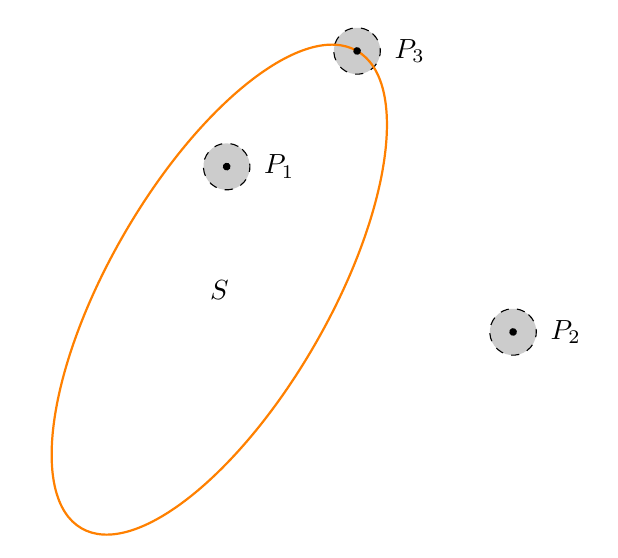
\begin{tikzpicture}[scale=.7]
\filldraw[rotate=60,draw=black,dashed,fill=gray!40]
	(2,1)circle(12pt)
	(2,-5)circle(12pt)
	(5,0)circle(12pt);
\draw[orange,rotate=60,thick](0,0)ellipse[x radius=5,y radius=2];
\draw (0,0)node{\(S\)};
\fill[rotate=60]
	(2,1)circle(2pt)node[right=10pt]{\(P_1\)}
	(2,-5)circle(2pt)node[right=10pt]{\(P_2\)}
	(5,0)circle(2pt)node[right=10pt]{\(P_3\)};
\end{tikzpicture}
\caption{平面上的点与点集的关系}
\label{figure:集合论.平面上的点与点集的关系}
\end{figure}
\end{definition}

\begin{property}
设点集\(S\subseteq\mathbb{R}^2\).
任意一点\(P\in\mathbb{R}^2\)要么是\(S\)的内点,要么是\(S\)的外点,要么是\(S\)的边界点.

换言之,任意点集\(S\)的内点、外点和边界点的集合均无交集,即:
\begin{enumerate}
\item \(I(S) \cap E(S) = \emptyset\).
\item \(\partial{S} \cap I(S) = \emptyset\).
\item \(\partial{S} \cap E(S) = \emptyset\).
\end{enumerate}
\end{property}

\begin{definition}
设点\(P\)和点集\(S\)满足\(P \in S\).
定义:若\(\exists \mathring{U}(P)\)使得\[
\mathring{U}(P) \cap S = \emptyset,
\]则称\(P\)为\(S\)的\DefineConcept{孤立点}(acnode),记作\(P \in A(S)\).
\end{definition}

\begin{property}
\(S\)的内点必属于\(S\),即\[
P \in I(S) \implies P \in S
\]或\[
I(S) \subseteq S.
\]
\begin{proof}
\[
\left. \begin{array}{r}
P \in I(S) \iff \exists U(P) :\: U(P) \subseteq S \\
P \in U(P)
\end{array} \right\}
\implies P \in S.
\qedhere
\]
\end{proof}
\end{property}

\begin{property}
\(S\)的外点必不属于\(S\),即\(P \in E(S) \implies P \notin S\).
\begin{proof}
\begin{align*}
\left. \begin{array}{r}
P \in E(S) \iff \exists U(P) :\: U(P) \cap S = \emptyset \\
P \in U(P) \iff \{P\} \subseteq U(P) \implies \{P\} \cap S \subseteq U(P) \cap S
\end{array} \right\}
\implies& \{P\} \cap S \subseteq \emptyset \\
\implies \{P\} \cap S = \emptyset
\implies P \notin S.&
\qedhere
\end{align*}
\end{proof}
\end{property}

\begin{example}
点集的边界点可能属于该点集,也可能不属于它.例如,实轴上的左闭右开区间\([a,b)\)有两个边界点\(a\)和\(b\),但\(a \in [a,b)\)而\(b \notin [a,b)\).
\end{example}

\begin{definition}
设点\(P\in\mathbb{R}^2\),点集\(S\subseteq\mathbb{R}^2\).
定义:如果点\(P\)的任意邻域内总有\(S\)中的无穷多个点,则称\(P\)是\(S\)的\DefineConcept{聚点}(cluster),记作\(P \in C(S)\),即\[
P \in C(S)
\iff
\forall\delta>0,\exists Q \in S : Q \in \mathring{U}(P,\delta).
\]称点集\(S\)的聚点的集合\(C(S)\)为\(S\)的\DefineConcept{导集}(derived set).
\end{definition}
任取点集\(S\)的一个聚点\(P_C\).由聚点的定义可知,\(P_C\)可以属于\(S\),也可以不属于\(S\).

\begin{theorem}
点\(P\)是点集\(S\)的聚点的充要条件是:在\(P\)的任意邻域内总有异于点\(P\)而属于\(S\)的一个点,即\[
\forall \delta>0 \bigl[
	\mathring{U}(P,\delta) \cap S \neq \emptyset
\bigr].
\]
\end{theorem}

\begin{property}
点集的内点均是其聚点,即\(I(S) \subseteq C(S)\).
\begin{proof}
由内点的定义有\(P \in I(S) \iff \exists \delta_1>0 :\: U(P,\delta_1) \subseteq S\).

当\(0 < \delta_2 \leqslant \delta_1\)时,有\[
\mathring{U}(P,\delta_2)
\subseteq U(P,\delta_1)
\subseteq S,
\]所以\[
\mathring{U}(P,\delta_2) \cap S
= \mathring{U}(P,\delta_2)
\neq \emptyset.
\]

当\(\delta_2 > \delta_1\)时,有\[
\emptyset \neq \mathring{U}(P,\delta_1) \subsetneqq U(P,\delta_1) \subseteq S,
\]\[
\mathring{U}(P,\delta_2) \cap S
\supseteq \mathring{U}(P,\delta_1) \cap S \neq \emptyset.
\]

综上所述,对于\(\forall \delta_2 > 0\)都有\(\mathring{U}(P,\delta_2) \cap S \neq \emptyset\)成立,即\(P \in C(S)\).
\end{proof}
\end{property}

\begin{property}
点集的外点不是其聚点,即\(P \in E(S) \implies P \notin C(S)\).
\begin{proof}
因为\(P \in E(S)\),所以\(\exists \delta > 0: U(P,\delta) \cap S = \emptyset\).又因为\(\mathring{U}(P,\delta) \subsetneqq U(P,\delta)\),所以\[
U(P,\delta) \cap S \supsetneqq \mathring{U}(P,\delta) \cap S = \emptyset,
\]从而有\(P \notin C(S)\).
\end{proof}
\end{property}

\begin{property}
点集的孤立点不是聚点,即\(P \in A(S) \implies P \notin C(S)\).
\begin{proof}
\(P \in A(S) \implies \exists \delta > 0 : \mathring{U}(P,\delta) \cap S = \emptyset \iff P \notin C(S)\).
\end{proof}
\end{property}

\begin{property}
点集的孤立点必不是其内点,点集的内点也必不是其孤立点,即\[
P \in A(S) \implies P \notin I(S),
\]\[
P \in I(S) \implies P \notin A(S).
\]
\end{property}

\begin{property}
点集的孤立点必不是其外点,点集的外点也必不是其孤立点,即\[
P \in A(S) \implies P \notin E(S),
\]\[
P \in E(S) \implies P \notin A(S).
\]
\end{property}

\begin{property}
点集的孤立点必是其边界点,即\(A(S) \subseteq \partial{S}\).
\end{property}

\begin{property}
点集的边界点可能是聚点,也可能不是聚点.
\end{property}

\begin{definition}
设点集\(S \subseteq \mathbb{R}^2\).

若\(S\)的点皆为它的内点,则称\(S\)为\DefineConcept{开集}.若\(S\)的所有边界点都属于\(S\)(即\(\partial S \subseteq S\)),或所有聚点皆属于\(S\)(即\(C(S) \subseteq S\)),则称\(S\)为\DefineConcept{闭集}.

若\(\exists r > 0\),使得\[
S \subseteq U(O,r),
\]其中\(O\)是坐标原点\(\opair{0,0}\),则称“\(S\)是\DefineConcept{有界的}”或“\(S\)是\DefineConcept{有界集}”;
否则称“\(S\)是\DefineConcept{无界的}”或“\(S\)是\DefineConcept{无界集}”.

若\(S\)中任意两点均可用一条全含于\(S\)内的折线相连接,则称“\(S\)是\DefineConcept{连通的}”或“\(S\)是\DefineConcept{连通集}”.

若\(S\)既是连通集又是开集,则称\(S\)为\DefineConcept{开区域}.
开区域\(S\)及其边界\(\partial S\)的并集\(S + \partial S\)称为\DefineConcept{闭区域}%
(简称\DefineConcept{闭域},常记作\(\overline{S}\)).
开区域与闭区域统称\DefineConcept{区域}.
\end{definition}

\begin{definition}\label{definition:集合论.平面区域的连通性}
%@see: https://mathworld.wolfram.com/SimplyConnected.html
%@see: https://mathworld.wolfram.com/MultiplyConnected.html
如果在平面区域\(S \subseteq \mathbb{R}^2\)内,%
任一闭曲线所围的部分都属于\(S\),%
则称“平面区域\(S\)是\DefineConcept{单连通的}(simply-connected)”;
否则称“平面区域\(S\)是\DefineConcept{复连通的}(multiply-connected)”.
\end{definition}










\section{数理逻辑概论}
\subsection{命题的概念}
\begin{definition}
\DefineConcept{命题}(proposition),%
是指对确定的对象进行判断的“陈述句”.
我们常用小写字母(如\(p,q\)等)表记命题.
\end{definition}

\begin{definition}
如果命题\(p\)的判断正确,%
那么我们称“命题\(p\)是\DefineConcept{真的}(true)”,%
或称“命题\(p\)是\DefineConcept{真命题}”,
或称“;
如果命题\(p\)的判断错误,%
那么我们称“命题\(p\)是\DefineConcept{假的}(false)”,%
或称“命题\(p\)是\DefineConcept{假命题}”.
\end{definition}

对于一个命题,它要么是真命题,要么是假命题.
悖论不能作为命题.

我们可以用集合表示命题的真值.
一般用空集\(\emptyset\)表示假命题,%
用任意非空集(例如\(\Set{\emptyset}\))表示真命题.

我们也可以用数字表示命题的真值.
一般用\(0\)表示假命题,%
用任意非零整数(例如\(1\))表示真命题.

\begin{definition}
\DefineConcept{逻辑联结词}(logical connectives),%
是指连接命题,对各个命题的真值进行运算的词,%
例如“\emph{且}”“\emph{或}”“\emph{不}”“\emph{非}”%
“\emph{如果……那么……}”“\emph{当且仅当}”等.
\end{definition}

为了将逻辑联结词形式化,我们可以使用符号来代表逻辑联结词.

\begin{table}[bp]
\centering
\begin{tabular}{|*{3}{c|}}
\hline
{\bf 概念} & {\bf 意义} & {\bf 符号} \\ \hline
{\bf 否定词}(negative) & 不、非 & \(\neg\) \\ \hline
{\bf 合取词}(conjunction) & 且、而且、并且 & \(\land\) \\ \hline
{\bf 析取词}(disjunction) & 或、或者 & \(\lor\) \\ \hline
{\bf 蕴涵词}(implication) & 如果……那么…… & \(\implies\) \\ \hline
{\bf 等价词}(equivalence) & 当且仅当 & \(\iff\) \\ \hline
\end{tabular}
\caption{逻辑联结词}
\end{table}

\begin{definition}
\DefineConcept{简单命题}或\DefineConcept{原子命题}(atom proposition),%
是指不含有逻辑联结词的命题.
相反地,\DefineConcept{复合命题}(compound proposition),%
是指包含了简单命题和逻辑联结词的命题.
\end{definition}

逻辑联结词具有对命题的真值进行运算的效果,%
我们可以用\DefineConcept{真值表}来说明其具体效果.

\begin{table}[ht]
\centering
\begin{subtable}[ht]{0.9\textwidth}
\centering
\begin{tabular}{|c|p{1.5cm}|}
\hline
\(p\) & \(\neg p\) \\ \hline
0 & 1 \\ \hline
1 & 0 \\ \hline
\end{tabular}
\caption{否定词“非”}
\end{subtable}

\begin{subtable}[ht]{0.45\textwidth}
\centering
\begin{tabular}{|*{2}{c|}p{2cm}|}
\hline
\(p\) & \(q\) & \(p \land q\) \\ \hline
0 & 0 & 0 \\ \hline
0 & 1 & 0 \\ \hline
1 & 0 & 0 \\ \hline
1 & 1 & 1 \\ \hline
\end{tabular}
\caption{合取词“且”}
\end{subtable}
\begin{subtable}[ht]{0.45\textwidth}
\centering
\begin{tabular}{|*{2}{c|}p{2cm}|}
\hline
\(p\) & \(q\) & \(p \lor q\) \\ \hline
0 & 0 & 0 \\ \hline
0 & 1 & 1 \\ \hline
1 & 0 & 1 \\ \hline
1 & 1 & 1 \\ \hline
\end{tabular}
\caption{析取词“或”}
\end{subtable}

\begin{subtable}[ht]{0.45\textwidth}
\centering
\begin{tabular}{|*{2}{c|}p{2cm}|}
\hline
\(p\) & \(q\) & \(p \implies q\) \\ \hline
0 & 0 & 1 \\ \hline
0 & 1 & 1 \\ \hline
1 & 0 & 0 \\ \hline
1 & 1 & 1 \\ \hline
\end{tabular}
\caption{蕴涵词}
\end{subtable}
\begin{subtable}[ht]{0.45\textwidth}
\centering
\begin{tabular}{|*{2}{c|}p{2cm}|}
\hline
\(p\) & \(q\) & \(p \iff q\) \\ \hline
0 & 0 & 1 \\ \hline
0 & 1 & 0 \\ \hline
1 & 0 & 0 \\ \hline
1 & 1 & 1 \\ \hline
\end{tabular}
\caption{等价词}
\end{subtable}

\caption{单个逻辑联结词逻辑运算结果的真值表}
\end{table}

\begin{definition}
如果有“\(p\)成立时\(q\)必成立”,%
记\(p \implies q\),%
称“\(p\)是\(q\)的\DefineConcept{充分条件}”,%
或称“\(q\)是\(p\)的\DefineConcept{必要条件}”;
分别称\(p\)和\(q\)为这个命题的\DefineConcept{蕴含前件}和\DefineConcept{蕴含后件}.
\end{definition}

在自然语言中,条件语句一般都具有内在的联系;
而数理逻辑中的\emph{蕴含}则仅是命题的连接,不一定具有什么内在联系.

\begin{property}
只有当“\(p\)为真,且\(q\)为假”时,蕴含式\(p \implies q\)才为假.
\end{property}
可以观察发现,\(p \implies q\)的真值表与\(\neg p \land q\)的相同.

\subsection{命题公式及其组成成分}
\begin{definition}
\DefineConcept{命题常元}(proposition constant),%
简称\DefineConcept{常元}(constant),%
表示具体命题.
\DefineConcept{命题变元}(proposition variable),%
简称\DefineConcept{变元}(variable),%
表示以“真、假”或者“0、1”为取值范围的变量.
\end{definition}

\begin{definition}
\DefineConcept{命题公式}(proposition formula),%
简称为\DefineConcept{公式}(formula),%
是指由命题常元、命题变元和逻辑联结词组成的命题.
它有如下的归纳定义:
\begin{enumerate}
\item 命题常元和命题变元是命题公式,也称作\DefineConcept{原子公式}或\DefineConcept{原子};
\item 设\(A\)、\(B\)为命题公式,那么有\[
(\neg A),\quad
(A \land B),\quad
(A \lor B),\quad
(A \implies B),\quad
(A \iff B)
\]也都是命题公式;
\item 只有有限步地引用上述两条所组成的符号串,才是命题公式.
\end{enumerate}
\end{definition}

\begin{example}
根据定义,\((\neg(p \implies (q \land r)))\)是命题公式.
\((qp)\)缺少联结词,所以不是命题公式.
\((p_1 \land (p_2 \land \dotsb))\)是无限的,所以不是命题公式.
\end{example}

为了简化书写,我们可以规定逻辑联结词的优先级顺序.
逻辑联结词的优先级为:\[
\neg,\quad \land,\quad \lor,\quad \implies,\quad \iff.
\]除非有括号,否则按照命题公式从左到右,按照优先级从高到低的次序结合.
定义逻辑联结词的优先级的意义在于可以减少命题公式中的括号数量.

\begin{example}
\(((\neg p) \lor (q))\)等同于\(\neg p \lor q\).

但\[
	p \implies q \land r \implies s
\]并非\[
	((p \implies q) \land (r \implies s)),
\]而应等同于\[
	((p \implies (q \land r)) \implies s).
\]
\end{example}

\begin{definition}
如果对于一个公式,不论其命题变元取何值,该公式总为真,%
则称该公式为\DefineConcept{永真式}或\DefineConcept{重言式}.
\end{definition}

常见的永真式列举如下:\begin{enumerate}
\item 肯定后件律 \(p \implies (q \implies p)\);
\item 同一律 \(p \implies p\);
\item 排中律 \(\neg p \lor p\);
\item 矛盾律 \(\neg(\neg p \land p)\);
\item 双重否定律 \(\neg\neg p \iff p\).
\end{enumerate}
